 

 
 

\chapter{Limits of   Functions and Continuity}\label{ch2}

 In this chapter, we study functions $f:D\rightarrow \mathbb{R}$ defined on a subset of real numbers $D$, and taking values in the set of real numbers $\mathbb{R}$. 
 Polynomials and rational functions are special examples.  When we do not specify the domain of a function, we will take its domain $D$ to be the largest subset of real numbers where the function can be defined.
 
 \begin{definition}{Polynomials and Rational Functions}
 A polynomial is a function $p:\mathbb{R}\rightarrow\mathbb{R}$ of the form
 \[p(x)=a_nx^n+a_{n-1}x^{n-1}+\ldots+a_1x+a_0,\]
 where $a_0, a_1, \ldots, a_n$ are constants. We call $p(x)$ a polynomial of degree $n$ if $a_n\neq 0$. 
 A rational function is a function of the form 
 \[f(x)=\frac{p(x)}{q(x)},\]
 where $p(x)$ and $q(x)$ are polynomials, and $q(x)$ is not the zero polynomial. The domain of this function is the set $D=\mathbb{R}\setminus S$, where $S$ is the finite point set containing all $x$ for which $q(x)=0$.
 \end{definition}
 
 For example, the domain of the rational function \[ f(x)=\frac{x^2+1}{x+2}\] is the set $D=\mathbb{R}\setminus\{-2\}$.
 
 
 To be able to apply tools in analysis, we are   interested in functions that are continuous. 
 Continuity can be defined in two different  ways that are equivalent. One is using positive numbers $\delta$ and $\varepsilon$ to measure distances of points in the domain and range, while the other is using limits of sequences. 
 
 The limit of a function $f:D\rightarrow \mathbb{R}$ when the variable $x$ approaches a limit point $x_0$ of the domain $D$ is an important concept in defining derivatives.  This concept can be defined for any function $f:D\rightarrow \mathbb{R}$ whose domain $D$ contains limit points. 
 There is a close relation between the limit of a function $f(x)$ when $x$ approaches a limit point $x_0$, and the continuity of the function at $x_0$. 
 
 Although the continuity of a function can be defined independently of limits of functions, we choose to consider limits of functions first. 
 
\section{Limits of Functions }\label{sec2.1 }

 In Section \ref{sec1.6}, we have defined the concept of limit points of a set $D$. The point $x_0$ is a limit point of the set $D$ if there is a sequence of points in $D\setminus\{x_0\}$ that converges to $x_0$. A limit point of a set is not necessarily in that set. A set that contains all its limit points is a closed set. If a point $x_0$ is in a set $D$ but is not a limit point of $D$, it is called an isolated point of $D$. If $x_0$ is an isolated point of $D$, there is a neighbourhood $(a,b)$ of $x_0$ which intersects the set $D$ only at the point $x_0$.
 
 Limits of functions can be defined using the $\varepsilon-\delta$ language or using limits of sequences. We will define the concept using limits of sequences first, and then show that it is equivalent to the $\varepsilon-\delta$  definition.
 
 \begin{definition} 
 {Limits of   Functions}
 Let $D$ be a subset of real numbers and let $x_0$ be a limit point of $D$. Given a function $f:D\rightarrow \mathbb{R}$, we say that {\it the limit of $f(x)$ as $x$ approaches $x_0$ is $\ell$}, provided that whenever $\{x_n\}$ is a sequence of points in $D\setminus\{x_0\}$ that converges to $x_0$, the sequence $\{f(x_n)\}$ converges to $\ell$. 
 
If the limit of $f:D\rightarrow \mathbb{R}$ as $x$ approaches $x_0$ is $\ell$, we write
 \[\lim_{x\rightarrow x_0}f(x)=\ell.\]
 \end{definition}
 Notice that we do not define $\di\lim_{x\rightarrow x_0}f(x)$ if $x_0$ is not a limit point of the domain where the function is defined. 
  
 \begin{highlight}{Logical Expression for Definition of  Limits}
 ~\vspace{-0.5cm}
 \begin{align*}
 & \lim_{x\rightarrow x_0}f(x)=\ell
 \iff \\& \forall  \{x_n\} \subset   D\setminus\{x_0\},\;\lim_{n\rightarrow \infty}x_n=x_0 \,\implies\,\lim_{n\rightarrow\infty}f(x_n)=\ell.\end{align*}
 \end{highlight}
 
 Let us first look at some examples. 
 \begin{example}{}
 Find the  limit if it exists.
 \begin{enumerate}[(a)]
 \item
 $\di\lim_{x\rightarrow 1}\frac{2x+3}{x^2+1}$
 
 \item $\di \lim_{x\rightarrow 1}\frac{x^2-1}{x-1}$
 
 \item $\di \lim_{x\rightarrow 1}\frac{x^2+1}{x-1}$
 \end{enumerate}
 \end{example}
 \begin{solution}{Solution}
 \begin{enumerate}[(a)]
 \item The function \[f(x)= \frac{2x+3}{x^2+1}\] is defined on $D=\mathbb{R}$. If $\{x_n\}$ is a sequence in $\mathbb{R}\setminus \{1\}$ that converges to 1, limit laws imply that
 \[\lim_{n\rightarrow\infty}f(x_n)=\lim_{n\rightarrow \infty}\frac{2x_n+3}{x_n^2+1}=\frac{2\times 1+3}{1^2+1}=\frac{5}{2}.\]Hence,
 \[\lim_{x\rightarrow 1}\frac{2x+3}{x^2+1}=\frac{5}{2}.\]\end{enumerate} \bs
 \begin{enumerate}[(b)] 
  \item The function \[f(x)= \frac{x^2-1}{x-1}\] is defined on $D=\mathbb{R}\setminus\{1\}$. If $\{x_n\}$ is a sequence in $\mathbb{R}\setminus \{1\}$ that converges to 1, limit laws imply that
 \[\lim_{n\rightarrow\infty}f(x_n)=\lim_{n\rightarrow \infty}\frac{x_n^2-1}{x_n-1}=\lim_{n\rightarrow \infty}(x_n+1)=2.\] Hence,
 \[\lim_{x\rightarrow 1}\frac{x^2-1}{x-1}=2.\]\end{enumerate}
 \begin{enumerate}[(c)]
 \item  The function \[f(x)= \frac{x^2+1}{x-1}\] is defined on $D=\mathbb{R}\setminus\{1\}$. Consider the sequence $\{x_n\}$ with 
 \[x_n=1+\frac{1}{n}.\]
 We find that \[f(x_n)=\frac{\di \frac{1}{n^2}+\frac{2}{n}+2}{\di \frac{1}{n}}=2n+2+\frac{1}{n}.\]The sequence $\{f(x_n)\}$ is not bounded, and so it is divergent. Hence, the limit
  \[\lim_{x\rightarrow 1}\frac{x^2+1}{x-1} \]does not exist.
 \end{enumerate}
 \end{solution}
 In part $(b)$, we have used the fact that $x_n\neq 1$  to simplify $f(x_n)$ to $x_n+1$. 
 
 Using   laws for limits of sequences, it is immediate to  see that limits of functions respect taking linear combinations and multiplications. It also respects taking quotients provided that the function on the denominator does not approach 0.
 
 \begin{proposition}[label=23020813]{Limit Laws for Functions}
Let $D$ be a subset of real numbers. Given that $f:D\rightarrow\mathbb{R}$ and $g:D\rightarrow\mathbb{R}$ are functions defined on $D$,   $x_0$ is a limit point of $D$,  and
\[\lim_{x\rightarrow x_0}f(x)=\ell_1,\hspace{1cm}\lim_{x\rightarrow x_0}g(x)=\ell_2.\]
\begin{enumerate}[1.]
\item
For any constants $\alpha$ and $\beta$, $\di \lim_{x\rightarrow x_0}(\alpha f+\beta g)(x)=\alpha\ell_1+\beta \ell_2$.
\item $\di \lim_{x\rightarrow x_0}(  f  g)(x)= \ell_1  \ell_2$.
\item If  $g(x)\neq 0$ for all $x\in D$, and $\ell_2\neq 0$, then
\[\lim_{x\rightarrow x_0}\frac{f(x)}{g(x)}=\frac{\ell_1}{\ell_2}.\]
\end{enumerate}
 \end{proposition}
 
 From this proposition, it follows that we can take limits of a rational function easily at a point which is not a zero of the polynomial in the denominator.
 \begin{proposition}[label=23020807]{}
 Let $p(x)$ and $q(x)$ be polynomials. If $x_0$ is a real number such that
 $q(x_0)\neq 0$, then
 \[\lim_{x\rightarrow x_0}\frac{p(x)}{q(x)}=\frac{p(x_0)}{q(x_0)}.\]
 \end{proposition}
 
 
 Let us now look at an example that involves the absolute values.
 \begin{example}[label=23020803]{}
 Show that for any real number $x_0$, 
 \[\lim_{x\rightarrow x_0}|x|=|x_0|.\]

\end{example}
\begin{solution}{Solution}
Let $\{x_n\}$ be a sequence in $\mathbb{R}\setminus\{x_0\}$ that converges to $x_0$. By Question \ref{absolute}, the sequence $\{|x_n|\}$ converges to $|x_0|$. This proves that
\[\lim_{x\rightarrow x_0}|x|=|x_0|.\]
\end{solution}

 Now we want to formulate an equivalent definition for limits.
 \begin{theorem}[label=23020801]{Equivalent Definitions for Limits}
  Let $D$ be a subset of real numbers, and let $x_0$ be a limit point of $D$. Given a function $f:D\rightarrow \mathbb{R}$, 
  the following are two equivalent definitions for 
  \[\lim_{x\rightarrow x_0}f(x)=\ell.\]  
  \begin{enumerate}[(i)]
  \item 
  Whenever $\{x_n\}$ is a sequence of points in $D\setminus\{x_0\}$ that converges to $x_0$, the sequence $\{f(x_n)\}$ converges to $\ell$. 
  \item For any $\varepsilon>0$, there is a $\delta>0$ such that if the point $x$ is in $D$ and $0<|x-x_0|<\delta$, then $|f(x)-\ell|<\varepsilon$.
  \end{enumerate} 
 \end{theorem}
 
 In logical notation, we can express (ii) as follows.
  \begin{highlight}{Logical Expression for Second Definition of  Limits}
 ~\vspace{-0.5cm}
 \begin{align*}
 & \lim_{x\rightarrow x_0}f(x)=\ell 
 \iff \\& \forall  \varepsilon>0, \;\exists \delta>0,\;\forall x\; (x\in D)\,\wedge (0<|x-x_0|<\delta)\;\implies \;|f(x)-\ell|<\varepsilon.\end{align*}
 \end{highlight}
 Here $\delta$ is a measure of the closeness of the point $x\in D$ to the point $x_0$, and $\varepsilon$ is a measure of the closeness of the function value $f(x)$ to the number $\ell$. The condition $|x-x_0|>0$ is to stress that we only consider those points $x$ that is not $x_0$. From the definitions, we can see that the limit of a function $f(x)$ when $x$ approaches $x_0$ does not depend on how the function $f $ is defined at $x_0$, and  $f$   does  not need to be defined at $x_0$ for the limit to be defined. 
 
 
 
 To prove Theorem \ref{23020801}, we need to show that (i) $\iff$ (ii). This is equivalent to (ii) $\implies$ (i) and $\neg$ (ii) $\implies$ $\neg$ (i). 
 \begin{myproof}{\linkt Proof of Theorem \ref{23020801}}
 We start by  showing that if (ii) holds, then (i) holds. Assume that (ii) holds. To prove (i), we take a sequence $\{x_n\}$ in $D\setminus\{x_0\}$ that converges to the point $x_0$. We want to show that the sequence $\{f(x_n)\}$ converges to $\ell$. We prove this using the definition of convergence of sequences. 
  Given $\varepsilon>0$, our assumption that (ii) holds implies that there is a $\delta>0$ such that for all $x$ that is in $D$ with $0<|x-x_0|<\delta$, we have $|f(x)-\ell|<\varepsilon$. Since $\{x_n\}$ converges to $x_0$, there is a positive integer $N$ such that for all $n\geq N$, $|x_n-x_0|<\delta$. By our definition, $x_n$ are points in $D\setminus \{x_0\}$. Hence, for all $n\geq N$,  
 \[|f(x_n)-\ell|<\varepsilon.\]Since we have shown that for all $\varepsilon>0$, there is a positive integer $N$ such that for all $n\geq N$, $|f(x_n)-\ell|<\varepsilon$, we conclude that the sequence $\{f(x_n)\}$ converges to $\ell$. This proves (i) holds.
 
Now assume that (ii) is false.  In logical notation, this means
\[\exists  \varepsilon>0, \;\forall \delta>0,\;\exists x\; (x\in D)\,\wedge (0<|x-x_0|<\delta)\;\wedge\;|f(x)-\ell|\geq \varepsilon.\] 
Namely, there is an $\varepsilon>0$ such that for any $\delta>0$, there is a point $x$ in $D\setminus\{x_0\}$ with $|x-x_0|<\delta$ but $|f(x)-\ell|\geq \varepsilon$.
For this $\varepsilon>0$, we  construct a sequence $\{x_n\}$ in $D\setminus \{x_0\}$ in the following way. For each positive integer $n$, there is a point $x_n$ in $D\setminus\{x_0\}$ such that
$|x_n-x_0|<1/n$ but $|f(x_n)-\ell|\geq\varepsilon$.
Then $\{x_n\}$ is a sequence in $D\setminus\{x_0\}$ that satisfies
\[|x_n-x_0|<\frac{1}{n}.\]
Since $\di\lim_{n\rightarrow \infty}1/n=0$, we find that the sequence $\{x_n\}$ converges to $x_0$. Since $|f(x_n)-\ell|\geq \varepsilon$ for all $n\in\mathbb{Z}^+$, the sequence $\{f(x_n)\}$ cannot converge to $\ell$. Hence, we have shown that there is a sequence $\{x_n\}$ in $D\setminus \{x_0\}$ that converges to $x_0$ but $\{f(x_n)\}$ does not converge to $\ell$. This proves that (i) does not hold.
 \end{myproof}
 
 \begin{example}[label=23020808]
 {The Heaviside Function}The Heaviside function  $H:\mathbb{R}\rightarrow\mathbb{R}$ is  defined by
 \begin{align*}
 H(x)=\begin{cases}1,\quad &\text{if}\; x\geq 0;
 \\0,\quad & \text{if}\;x<0.\end{cases}
 \end{align*}
 For any  real number $x_0$, determine whether the limit $\di\lim_{x\rightarrow x_0}H(x)$ exists.
 \end{example}
 
 \begin{figure}[ht]
\centering
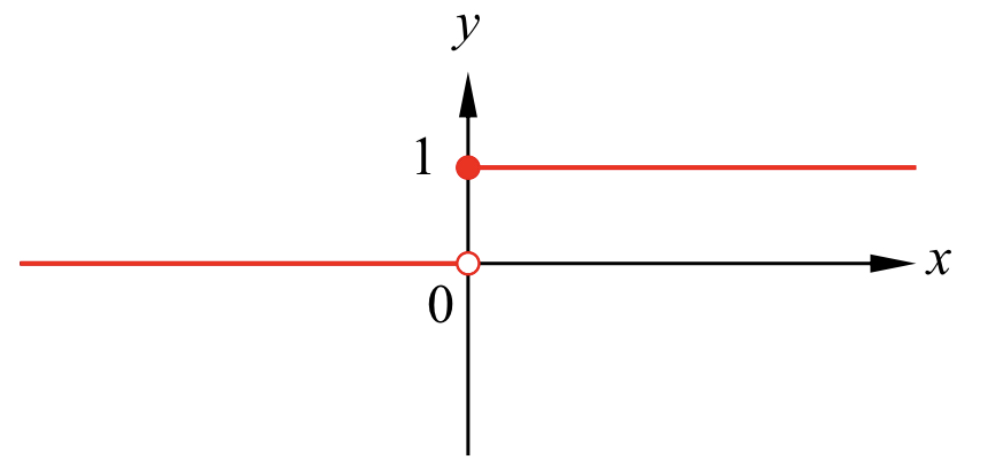
\includegraphics[scale=0.2]{Picture6.png}
\caption{  The Heaviside function $H(x)$.}\label{figure6}
\end{figure}


 \begin{solution}{Solution}
 We consider the cases where $x_0>0$, $x_0<0$ and $x_0=0$.
 
  \textbf{Case 1:} $x_0>0$.
 In this case, we claim that $\di\lim_{x\rightarrow x_0}f(x)=1$. \\Given $\varepsilon>0$, take $\delta=x_0$. Then $\delta>0$. If $x$ is in $\mathbb{R}$ and $0<|x-x_0|<\delta=x_0$, we have
 $x-x_0>-x_0$ and hence $x>0$. Thus $f(x)=1$ and 
 \[|f(x)-1|=0<\varepsilon.\]
 This proves that  $\di\lim_{x\rightarrow x_0}f(x)=1$.
 
 \textbf{Case 2:} $x_0<0$.
 In this case, we claim that $\di\lim_{x\rightarrow x_0}f(x)=0$. \\Given $\varepsilon>0$, take $\delta=-x_0$. Then $\delta>0$. If $x$ is in $\mathbb{R}$ and $0<|x-x_0|<\delta=-x_0$, we have
 $x-x_0<-x_0$ and hence $x<0$. Thus $f(x)=0$ and 
 \[|f(x)-0|=0<\varepsilon.\]
 This proves that  $\di\lim_{x\rightarrow x_0}f(x)=0$. 
 \bs
  \textbf{Case 3:} $x_0=0$.
 In this case, we claim that $\di\lim_{x\rightarrow x_0}f(x)$ does not exist. \
 Let $\{u_n\}$ and $\{v_n\}$ be the sequences $\{1/n\}$ and $\{-1/n\}$ respectively. They are both sequences in $\mathbb{R}\setminus\{0\}$ that converge to 0.
 \[f(u_n)=1 \quad\text{and}\quad f(v_n)=0 \hspace{1cm}\text{for all}\;n\in\mathbb{Z}^+.\]
 Therefore,
 \[\lim_{n\rightarrow\infty}f(u_n)=1\hspace{1cm}\text{and}\hspace{1cm}\lim_{n\rightarrow\infty}f(v_n)=0.\]
 Since $\{f(x_n)\}$ has different limits when we consider two different sequences $\{x_n\}$ in $\mathbb{R}\setminus\{0\}$ that converge to 0, we conclude that   $\di\lim_{x\rightarrow x_0}f(x)$ does not exist. 
 \end{solution}
 
 In this example, we can also use the $\varepsilon-\delta$ definition to show that  $\di\lim_{x\rightarrow  0}f(x)$ does not exist.  Assume that $\di\lim_{x\rightarrow  0}f(x)$ exists and is equal to $\ell$. Take $\varepsilon=1/2$. There exists $\delta>0$ such that for any $x\in \mathbb{R}$, if $0<|x-0|<\delta$, then
 \[|f(x)-\ell|<\varepsilon.\]Now the points $x=x_1=-\delta/2$ and $x=x_2=\delta/2$ both satisfy 
$0<|x-0|<\delta$. We have $f(x_1)=0$ and $f(x_2)=1$.
By triangle inequality,
\[|f(x_1)-f(x_2)|\leq |f(x_1)-\ell|+|f(x_2)-\ell|<2\varepsilon=1.\]
This gives
\[1=|f(x_1)-f(x_2)|<1,\]which is a contradiction. Hence, $\di\lim_{x\rightarrow 0}f(x)$ does not exist.
    

  
  In calculus, we have defined  the concepts of  left limits and right limits to deal with functions like the Heaviside function, which is defined by cases.
  Given a subset of real numbers $D$ and a point $x_0$, define
  \[D_{x_0, -}=\left\{x\in D\,|\,x< x_0\right\},\hspace{1cm} D_{x_0, +}=\left\{x\in D\,|\,x> x_0\right\}.\]
  For example, consider $D=[0, 2)$. If  $x_0=1$, then $D_{1,-}=[0,1)$ and $D_{1,+}=(1,2)$. If $x_0=0$, then $D_{0,-}=\emptyset$ and $D_{0,+}=(0,2)$. If $x_0=2$, then $D_{2,-}=[0,2)$ and $D_{2,+}=\emptyset$.
  
  Notice that even though $x_0$ is a limit point of $D$, it might not be a limit point of $D_{x_0,-}$ or $D_{x_0,+}$. 
  We define the left limit and right limit of a function $f:D\rightarrow\mathbb{R}$ when $x$ approaches $x_0$ in the following way.
  
  \begin{definition}{Left Limits and Right Limits}
   Let   $D$ be a subset of real numbers and let $f:D\rightarrow \mathbb{R}$ be a function defined on   $D$.  
   \begin{enumerate}[1.]
   \item If $x_0$ is a limit point of $D_{x_0,-}$, $D_{x_0,-}$ is not an empty set.  We say that the   limit of the function $f:D\rightarrow \mathbb{R}$ as $x$ approaches $x_0$ from the left exists provided that the limit of the function $f:D_{x_0,-}\rightarrow\mathbb{R}$ as $x$ approaches $x_0$ exists. If the left limit exists, it is denoted by
   \[\lim_{x\rightarrow x_0, x<x_0}f(x)\hspace{1cm}\text{or simply as}\hspace{1cm}\lim_{x\rightarrow x_0^-}f(x).\]
      \item If $x_0$ is a limit point of $D_{x_0,+}$, $D_{x_0,+}$ is not an empty set.  We say that the   limit of the function $f:D\rightarrow \mathbb{R}$ as $x$ approaches $x_0$ from the right exists provided that the limit of the function $f:D_{x_0,+}\rightarrow\mathbb{R}$ as $x$ approaches $x_0$ exists. If the right limit exists, it is denoted by
   \[\lim_{x\rightarrow x_0, x>x_0}f(x)\hspace{1cm}\text{or simply as}\hspace{1cm}\lim_{x\rightarrow x_0^+}f(x).\]
   \end{enumerate}
  
  \end{definition}
  
\begin{highlight}{Left Limits, Right Limits, and Limits}
\begin{enumerate}[1.]
\item If $x_0$ is a limit point of both $D_{x_0,+}$ and $D_{x_0,-}$, then $\di\lim_{x\rightarrow x_0}f(x)$ exists if and only if both $\di\lim_{x\rightarrow x_0^-}f(x)$ and $\di\lim_{x\rightarrow x_0^+}f(x)$ exist and they are equal. 
\item 
If $x_0$ is a limit point of $D_{x_0,-}$ but is not a limit point of $D_{x_0,+}$, then  $\di\lim_{x\rightarrow x_0}f(x)$ exists if and only if   $\di\lim_{x\rightarrow x_0^-}f(x)$ exists.
\item 
If $x_0$ is a limit point of $D_{x_0,+}$ but is not a limit point of $D_{x_0,-}$, then  $\di\lim_{x\rightarrow x_0}f(x)$ exists if and only if   $\di\lim_{x\rightarrow x_0^+}f(x)$ exists.
\end{enumerate}\end{highlight}
\begin{example}{}
For the Heaviside function, we have
  \[\lim_{x\rightarrow 0^-}H(x)=0\hspace{1cm}\text{and}\hspace{1cm}\lim_{x\rightarrow 0^+}H(x)=1.\]Since the left and right limits are not equal, $\di \lim_{x\to 0}H(x)$ dos not exist.\end{example}
  


 \begin{example}[label=23020809]
 {The Dirichlet's Function} The Dirichlet's function is the function $f:\mathbb{R}\rightarrow\mathbb{R}$ defined by
 \begin{align*}
 f(x)=\begin{cases}1,\quad &\text{if}\; x\;\text{is rational},
 \\0,\quad &\text{if}\; x\;\text{is irrational}.\end{cases}
 \end{align*}
 For any  real number $x_0$, determine whether the limit $\di\lim_{x\rightarrow x_0}f(x)$ exists.
 \end{example}This is a classical example of a function which we cannot visualize the graph.
 \begin{solution}{Solution}
 Fixed a real number $x_0$. For any positive integer $n$, there is a rational number $p_n$ and an irrational number $q_n$ in the open interval $(x_0-1/n, x_0)$. The sequences $\{p_n\}$ and $\{q_n\}$ are in $\mathbb{R}\setminus\{x_0\}$ and converge to $x_0$. Since
 \[f(p_n)=1\quad\text{and}\quad f(q_n)=0\hspace{1cm}\text{for all}\;n\in\mathbb{Z}^+,\]
 we find that 
 \[\lim_{n\rightarrow\infty}f(p_n)=1\hspace{1cm}\text{and}\hspace{1cm}\lim_{n\rightarrow\infty}f(q_n)=0.\]
 Since the sequence $\{f(x_n)\}$ has different limits when we consider two different sequences $\{x_n\}$ in $\mathbb{R}\setminus\{x_0\}$ that converge to $x_0$, we conclude that   $\di\lim_{x\rightarrow x_0}f(x)$ does not exist. 
 \end{solution}
 For this example, if one wants to use the $\varepsilon-\delta$ definition of limits, one can proceed in the following way. For fixed $x_0$ in $\mathbb{R}$, assume that  $\di\lim_{x\rightarrow x_0}f(x)=\ell$. When $\varepsilon=1/2$, there is a $\delta>0$ such that for any $x$ with $0<|x-x_0|<\delta$, $|f(x)-\ell|<\varepsilon$. The open interval $(x_0-\delta, x_0)$ contains a rational number $x_1$  and an irrational number $x_2$. Notice that $f(x_1)=1$ and $f(x_2)=0$.  Both $x=x_1$ and $x=x_2$ satisfy $0<|x-x_0|<\delta$. By triangle inequality,
\[|f(x_1)-f(x_2)|\leq |f(x_1)-\ell|+|f(x_2)-\ell|<2\varepsilon=1.\]
This gives
\[1=|f(x_1)-f(x_2)|<1,\]which is a contradiction. Hence, $\di\lim_{x\rightarrow x_0}f(x)$ does not exist.
 
Next, we consider composite functions. 
\begin{proposition}[label=23020815]{}
Given the two functions $f:D\rightarrow \mathbb{R}$ and $g: U\rightarrow\mathbb{R}$, if $f(D)\subset U$, we can define the composite function $h=g\circ f:D\rightarrow \mathbb{R}$ by
$h(x)=g(f(x))$. If $x_0$ is a limit point of $D$, $y_0$ is a limit point of $U$, $f(D\setminus\{x_0\})\subset U\setminus\{y_0\}$,
\[\lim_{x\rightarrow x_0}f(x)=y_0,\hspace{1cm}\lim_{y\rightarrow y_0}g(y)=\ell,\] then
\[\lim_{x\rightarrow x_0}h(x)=\lim_{x\rightarrow x_0}(g\circ f)(x)=\ell.\]
\end{proposition}
\begin{myproof}{Proof}
Let $\{x_n\}$ be a sequence in $D\setminus\{x_0\}$ that converges to $x_0$, and let $y_n=f(x_n)$ for all $n\in\mathbb{Z}^+$. By assumption,   $\{y_n\}$ is a sequence in $U\setminus\{y_0\}$.  Since $\di \lim_{x\rightarrow x_0}f(x)=y_0$, the sequence $\{f(x_n)\}$ converges to $y_0$. Since $\di\lim_{y\rightarrow y_0}g(y)=\ell$, the sequence
$\{g(y_n)\}$ converges to $\ell$. In other words, the sequence $\{(g\circ f)(x_n)\}$ converges to $\ell$.

Since we have proved that whenever  $\{x_n\}$ is a sequence in $D\setminus\{x_0\}$ that converges to $x_0$, the sequence $\{(g\circ f)(x_n)\}$ converges to $\ell$, we conclude that
\[\lim_{x\rightarrow x_0}(g\circ f)(x)=\ell.\]
\end{myproof}


Using the result of Example \ref{23020803}, we obtain the following.
\begin{corollary}{}
Let $D$ be a subset of real numbers. Given a function $f:D\rightarrow\mathbb{R}$, if $x_0$ is a limit point of $D$ and 
$\di \lim_{x\rightarrow x_0}f(x)=\ell$,
then
\[\lim_{x\rightarrow x_0}|f(x)|=|\ell|.\]
\end{corollary}

%Now let us consider the square-root function $f(x)=\sqrt{x}$, $x\geq 0$.
\begin{example}[label=23020901]{}
For any $x_0\geq 0$, show that
\[\lim_{x\rightarrow x_0}\sqrt{x}=\sqrt{x_0}.\]
\end{example}
\begin{solution}{Solution}
Let us use the $\varepsilon-\delta$ definition of limits. 
Consider the case $x_0=0$ first. Given $\varepsilon>0$, take $\delta=\varepsilon^2$. Then $\delta>0$. If $x\geq 0$ is such that $0<|x-0|<\delta=\varepsilon^2$, we have $0<x<\varepsilon^2$, which implies that
$\di 0< \sqrt{x}<\varepsilon$. Hence,  if $x\geq 0$ and $0<|x-0|<\delta$,
\[|\sqrt{x}-\sqrt{0}|<\varepsilon.\] This proves  that
\[\lim_{x\rightarrow 0}\sqrt{x}=0=\sqrt{x_0}.\]

Now consider the case $x_0>0$. 
Notice that
\[\sqrt{x}-\sqrt{x_0}=\frac{x-x_0}{\sqrt{x}+\sqrt{x_0}}.\]
 If $x>x_0/4$, then $\sqrt{x}>\sqrt{x_0}/2$ and
 \[\frac{1}{\sqrt{x}+\sqrt{x_0}}<\frac{2}{3\sqrt{x_0}}.\]
Given $\varepsilon>0$, let
$\di \delta=\min\left\{\frac{3}{4}x_0,\; \frac{3}{2}\varepsilon\sqrt{x_0} \right\}$.
Then $\delta>0$. If $x\geq 0$ and $0<|x-x_0|<\delta$, then $\di |x-x_0|<\frac{3}{4}x_0$ and so $\di x>\frac{1}{4}x_0$. 
Therefore,\bs
\[\left|\sqrt{x}-\sqrt{x_0}\right|=\frac{|x-x_0|}{\sqrt{x}+\sqrt{x_0}}<\delta\times \frac{2}{3\sqrt{x_0}}\leq\varepsilon.\]
This proves that 
$\di \lim_{x\rightarrow x_0}\sqrt{x} =\sqrt{x_0}$.
\end{solution}

\begin{figure}[ht]
\centering
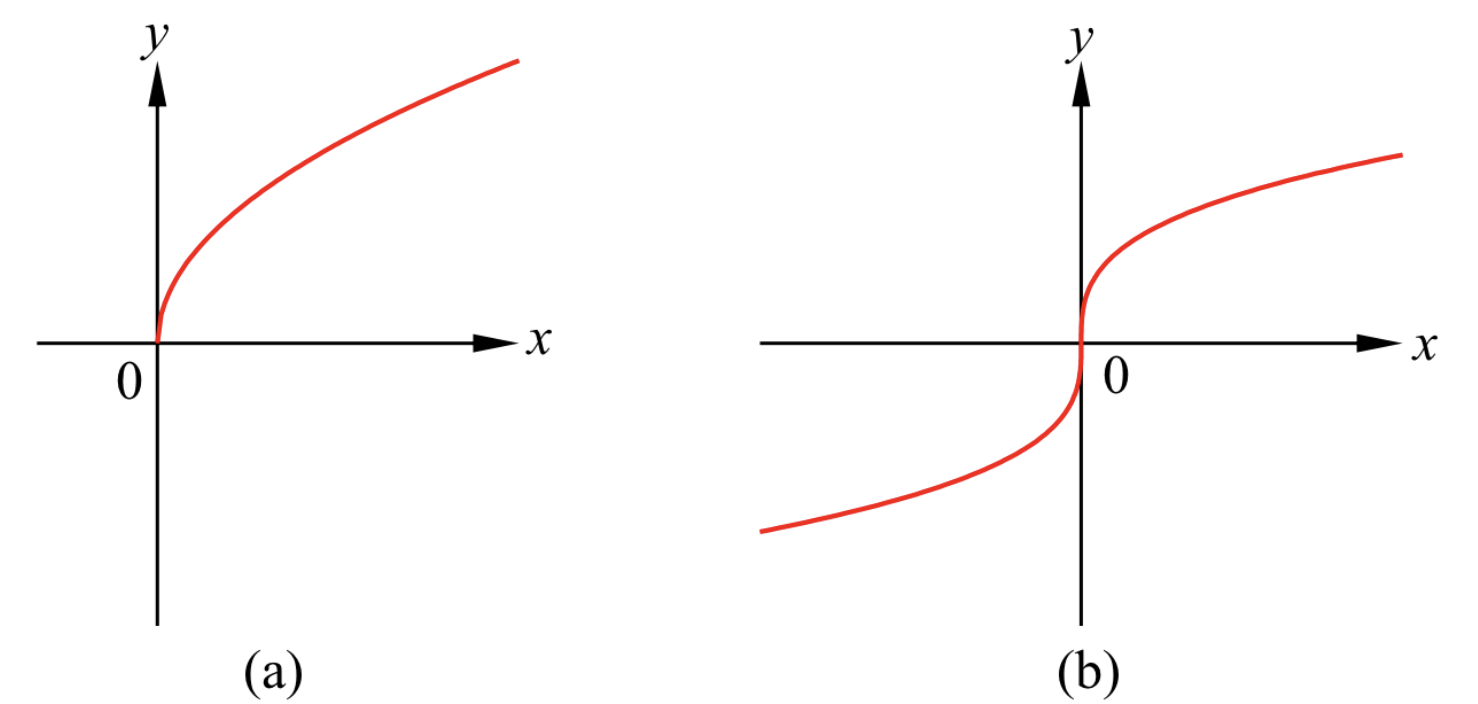
\includegraphics[scale=0.2]{Picture7.png}
\caption{  (a) The function $f(x)=\sqrt{x}$. (b) The function $f(x)=\sqrt[3]{x}$.}\label{figure7}
\end{figure}

Using similar methods, one can prove that  if $n$ is an   integer,   then for any $x_0$ in the domain of the function $f(x)=\sqrt[n]{x}$,
\[\lim_{x\rightarrow x_0}\sqrt[n]{x}= \sqrt[n]{x_0}.\]
 

Now we want to give a brief discussion about limits that involve infinities.  
\begin{definition}{Infinity as Limits of Sequences}
Given that $\{a_n\}$ is a sequence of real numbers.
\begin{enumerate}[1.]
\item
We say that the sequence $\{a_n\}$ diverges to $\infty$, written as
$\di \lim_{n\rightarrow \infty}a_n=\infty$,
if for every positive number $M$, there is a positive integer $N$ such that for all $n\geq N$,
$a_n\geq M$.
\item
We say that the sequence $\{a_n\}$ diverges to $-\infty$, written as
$\di \lim_{n\rightarrow \infty}a_n=-\infty$,
if for every positive number $M$, there is a positive integer $N$ such that for all $n\geq N$,
$a_n\leq -M$.
\end{enumerate}\end{definition}
 
\begin{example}{}
\begin{enumerate}[(a)]
\item
The sequence $\{n^2\}$ diverges to $\infty$.
\item The sequence $\{-n^2\}$ diverges to $-\infty$.
\item The sequence $\{(-1)^nn^2\}$ neither diverges to $\infty$ nor to $-\infty$.
\end{enumerate}
\end{example}
%Notice that the sequence $\{a_n\}$ diverges to $-\infty$ if and only if the sequence $\{-a_n\}$ diverges to $\infty$.

Given that $\{x_n\}$ is a sequence of  real numbers. If $\{x_n\}$ diverges to $\infty$ or $-\infty$, there is a positive integer $N$ such that $x_n\neq 0$ for all $n\geq N$. Hence, for sequences that diverge to $\infty$ and $-\infty$, we can assume none of the terms is zero.
 

The following is another characterization of boundedness for a set in terms of sequences that diverge to infinity.
\begin{highlight}{}

\begin{enumerate}[1.]
\item A set $D$ is not bounded above if and only if there is a sequence $\{x_n\}$ in $D$ that diverges to $\infty$. 
\item A set $D$ is not bounded below if and only if there is a sequence $\{x_n\}$ in $D$ that diverges to $-\infty$. 
\end{enumerate}
\end{highlight}

Using these, we can make the following definitions.
  
\begin{definition}{Limits of Functions at Infinity}
Let $D$ be a subset of real numbers that is not bounded above. Given  that $\ell$ is a real number and $f:D\rightarrow\mathbb{R}$  is a function  defined on the set $D$.  The following  two   definitions for
\[\lim_{x\rightarrow\infty}f(x)=\ell \]are equivalent.
\begin{enumerate}[(i)]
\item Whenever $\{x_n\}$ is a sequence of points in $D$ that diverges to $\infty$, the sequence $\{f(x_n)\}$ converges to  $\ell$. 
\item For any $\varepsilon>0$, there is a positive number $M  $ such that if the point $x$ is in $D$ and $x>M$, then
\[|f(x)-\ell|<\varepsilon.\]
\end{enumerate}
\end{definition}

\begin{definition}{Limits of Functions at Negative Infinity}
Let $D$ be a subset of real numbers that is not bounded below. Given  that $\ell$ is a real number and $f:D\rightarrow\mathbb{R}$  is a function  defined on the set $D$.  The following  are two equivalent definitions for
\[\lim_{x\rightarrow-\infty}f(x)=\ell.\]
\begin{enumerate}[(i)]
\item Whenever $\{x_n\}$ is a sequence of points in $D$ that diverges to $-\infty$, the sequence $\{f(x_n)\}$ converges to  $\ell$. 
\item For any $\varepsilon>0$, there is a positive number $M  $ such that if the point $x$ is in $D$ and $x<-M$, then
\[|f(x)-\ell|<\varepsilon.\]
\end{enumerate}
\end{definition}

Now let us look at a simple example.
\begin{example}[label=23020903]{}
Show that $\di\lim_{x\rightarrow\infty}\frac{1}{x}=0$.
\end{example}
\begin{solution}{Solution}
We use both definitions to prove the statement.

Using the sequence definition, let $\{x_n\}$ be a sequence of nonzero real numbers that diverges to $\infty$. We want to show that the sequence $\{1/x_n\}$ converges to 0. Given $\varepsilon>0$, the number $M=1/\varepsilon$ is also positive. Since the sequence $\{x_n\}$ diverges to $\infty$, there is a positive integer $N$ such that for all $n\geq N$, 
\[x_n>M=\frac{1}{\varepsilon}.\] In particular, for all $n\geq N$, $x_n>0$ and
$\di 0<\frac{1}{x_n}<\varepsilon$. This proves that the sequence $\{1/x_n\}$ converges to 0. Therefore, $\di \lim_{x\rightarrow\infty}\frac{1}{x}=0$. 



Now consider the definition in terms of $\varepsilon$. Given $\varepsilon>0$, let $M=1/\varepsilon$. Then $M$ is a positive number. If $x$ in $\mathbb{R}\setminus\{0\}$ is such that $x>M$, then
\[0<\frac{1}{x}<\frac{1}{M}=\varepsilon.\]
This proves that $\di\lim_{x\rightarrow\infty}\frac{1}{x}=0$.
\end{solution}


This example demonstrates that working with the definition in terms of $\varepsilon$ is sometimes easier.

 \begin{figure}[ht]
\centering
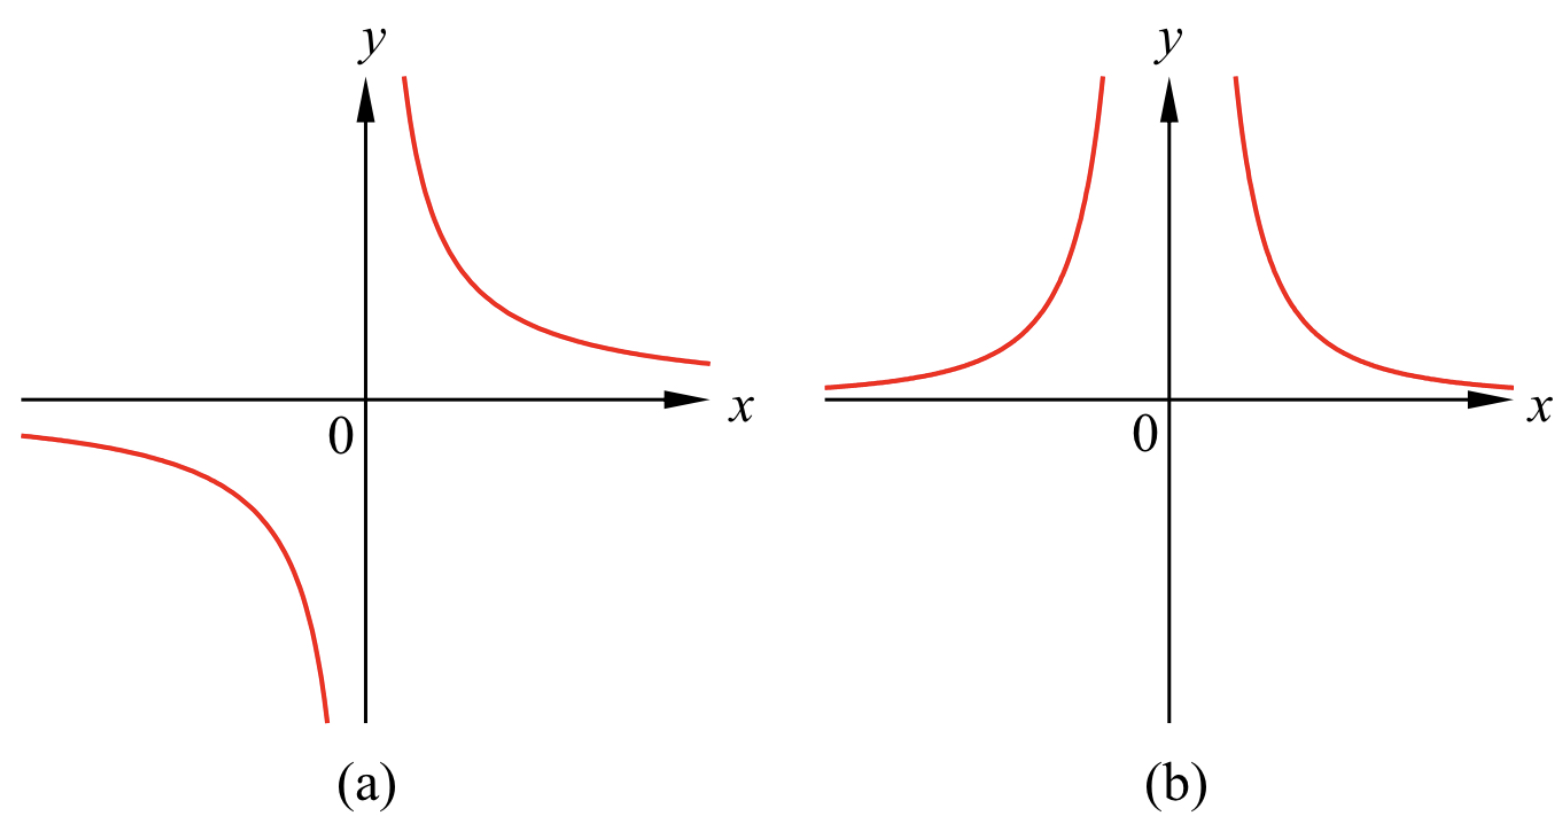
\includegraphics[scale=0.2]{Picture8.png}
\caption{  (a) The function $f(x)=1/x$. (b) The function $f(x)=1/x^2$.}\label{figure8}
\end{figure}

It is easy to see that the limit laws given in Proposition \ref{23020813} and Proposition \ref{23020815} also hold for the case where $x\rightarrow \infty$ or $x\rightarrow -\infty$. We will skip the formulation and use it directly. For example, we have the following.

\begin{example}{}
For any positive integer $n$, 
$\di \lim_{x\rightarrow\infty}\frac{1}{x^n}=0$.
\end{example}

Now let us look at some more examples.
\begin{example}{}
Determine whether the limit 
\[ \lim_{x\rightarrow\infty}\frac{2x^2+3x+4}{x^2+7}\]exists. If it  exists, find the limit.
 
\end{example}
\begin{solution}{Solution}
  Divide the numerator and denominator by $x^2$, we have
\[\frac{2x^2+3x+4}{x^2+7}=\frac{2+\di\frac{3}{x}+\frac{4}{x^2}}{1+\di\frac{7}{x^2}}.\]
Using limit laws and the fact that $\di\lim_{x\rightarrow\infty}1/x=0$, we find that
\[\lim_{x\rightarrow\infty}\frac{2x^2+3x+4}{x^2+7}=\frac{2+0+0}{1+0}=2.\]
 
\end{solution}

\begin{example}{}
Determine whether the limit 
\[  \lim_{x\rightarrow -\infty}\frac{x}{\sqrt{x^2+1}}\]exists. If it  exists, find the limit.

\end{example}

\begin{solution}{Solution}
  Notice that $\sqrt{x^2}=|x|$. Hence,
\[\frac{x}{\sqrt{x^2+1}}=\frac{x}{|x|\sqrt{1+\di\frac{1}{x^2}}}.\] 
When $x<0$, 
\[\frac{x}{|x|}=-1.\] 
Therefore,
\[\lim_{x\rightarrow-\infty}\frac{x}{|x|}=-1.\]On the other hand, since 
\[\lim_{x\rightarrow\infty}1+\di\frac{1}{x^2}=1\hspace{1cm}\text{and}\hspace{1cm}\lim_{y\rightarrow 1}\sqrt{y}=1,\] we find that
\[\lim_{x\rightarrow\infty}\frac{1}{\sqrt{1+\di\frac{1}{x^2}}}=1.\]Hence,
\[\lim_{x\rightarrow -\infty}\frac{x}{\sqrt{x^2+1}}=-1.\]
 
 
\end{solution}

 \begin{figure}[ht]
\centering
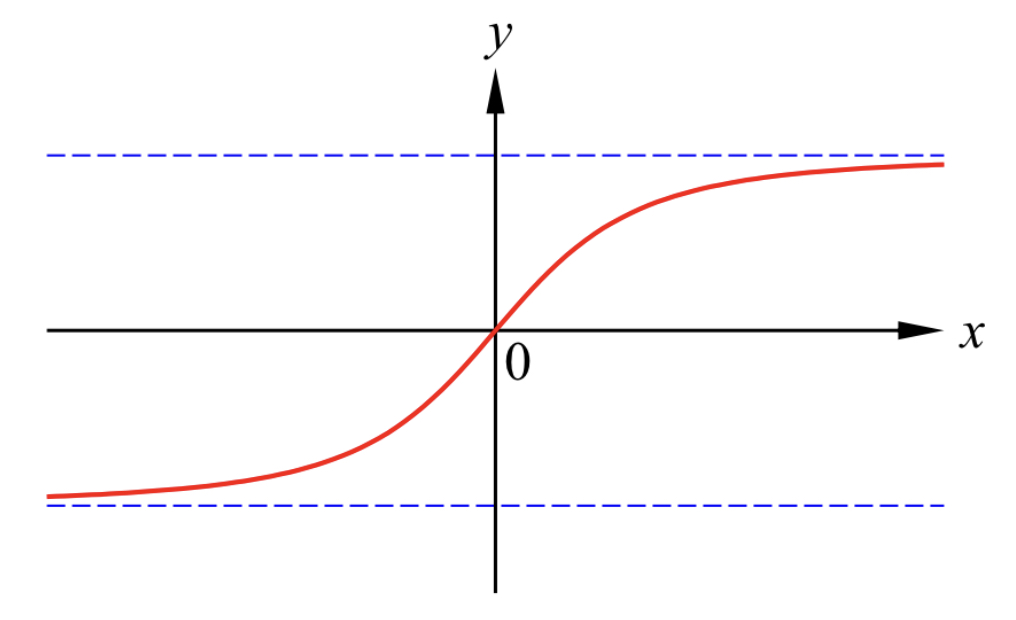
\includegraphics[scale=0.2]{Picture9.png}
\caption{  The function $\di f(x)=\frac{x}{\sqrt{x^2+1}}$.}\label{figure9}
\end{figure}

\begin{remark}{}
Using similar ideas, one can formulate analogous definitions for the following limits.
\[
 \lim_{x\rightarrow x_0}f(x)=\infty,\hspace{1cm}
 \lim_{x\rightarrow x_0}f(x)=-\infty,\]
\[\lim_{x\rightarrow \infty}f(x)=\infty,\hspace{1cm}
 \lim_{x\rightarrow \infty}f(x)=-\infty,\]
 \[
 \lim_{x\rightarrow -\infty}f(x)=\infty,\hspace{1cm}
 \lim_{x\rightarrow -\infty}f(x)=-\infty.\]
 
\end{remark}

Finally, we would like to mention that there is an analogue of the squeeze theorem for functions, whose proof is straightforward.
\begin{theorem}{Squeeze Theorem}
Let $D$ be a subset of real numbers. Given that   $f:D\rightarrow\mathbb{R}$, $g:D\rightarrow\mathbb{R}$, $h:D\rightarrow\mathbb{R}$ are functions defined on $D$ and
\[g(x)\leq f(x)\leq h(x)\hspace{1cm}\text{for all}\;x\in D.\]
If $x_0$ is a limit point of $D$ and
\[\lim_{x\rightarrow x_0}g(x)=\lim_{x\rightarrow x_0}h(x)=\ell,\]then
\[\lim_{x\rightarrow x_0}f(x)=\ell.\]
\end{theorem}

\sbr
\noindent
{\bf \large Exercises  \thesection}
\setcounter{myquestion}{1}



 \begin{question}{\themyquestion}
  Find the limit if it exists.
 \begin{enumerate}[(a)]
 \item
 $\di\lim_{x\rightarrow -1}\frac{x^2+3x+2}{x^2+1}$
 
 \item $\di \lim_{x\rightarrow -1}\frac{x^2-3x-4}{x+1}$
 
 \item $\di \lim_{x\rightarrow -1}\frac{x^2+1}{x+1}$
 
 \item  $\di \lim_{x\rightarrow -1}\left|\frac{x^2-3x-4}{x+1}\right|$
 \end{enumerate}
\end{question}
\atc
\begin{question}{\themyquestion}
  Define the function $f:\mathbb{R}\rightarrow\mathbb{R}$   by
 \begin{align*}
 f(x)=\begin{cases}x+3,\quad & \text{if}\; x\geq 1,
 \\5-x,\quad & \text{if}\;x<1.\end{cases}
 \end{align*}
 For any  real number $x_0$, determine whether the limit $\di\lim_{x\rightarrow x_0}f(x)$ exists.
\end{question}

\atc
\begin{question}{\themyquestion}
 Define the function $f:\mathbb{R}\rightarrow\mathbb{R}$   by
 \begin{align*}
 f(x)=\begin{cases}x,\quad & \text{if}\; x\;\text{is rational};
 \\-x,\quad & \text{if}\;x\;\text{is irrational}.\end{cases}
 \end{align*}
 \begin{enumerate}
 [(a)]
 \item Use squeeze theorem to show that  $\di\lim_{x\rightarrow 0}f(x)$ exists and find the limit.
 \item If $x_0\neq 0$, show that  $\di\lim_{x\rightarrow x_0}f(x)$ does not exist.
 \end{enumerate}
\end{question}

\atc

\begin{question}{\themyquestion}
Determine whether the limit exists. If it  exists, find the limit.
\begin{enumerate}[(a)]
\item[(a)]
$\di \lim_{x\rightarrow -\infty}\frac{2x^2+x+4}{5x^2+2}$
\item [(b)]$\di \lim_{x\rightarrow \infty}\frac{2x+3}{\sqrt{4x^2+1}}$
\end{enumerate}
\end{question}

\atc
\begin{question}{\themyquestion}
For any $x_0\geq 0$, show that
\[\lim_{x\rightarrow x_0}\sqrt[4]{x}=\sqrt[4]{x_0}.\]
\end{question}

\vp

\section{Continuity of Functions}\label{sec2.2}

In this section, we introduce the concept of continuity of functions.



\begin{definition}{Continuity}
Let $D$ be a subset of real numbers that contains the point $x_0$, and let $f:D\rightarrow\mathbb{R}$ be a function defined on $D$. We say that the function $f$ is {\bf continuous at } $x_0$ provided that whenever $\{x_n\}$ is a sequence of points in $D$ that converges to $x_0$, the sequence $\{f(x_n)\}$ converges to $f(x_0)$. 

We say that $f:D\rightarrow \mathbb{R}$ is a \textbf{continuous function} if it is continuous at every point of its domain $D$.
\end{definition}

The  definitions of limit and continuity are very similar. However, there is a slight difference. To define continuity at a point $x_0$, $x_0$ must be a point in the domain of the function $D$. To define limit, $x_0$ does not need to be a point in the domain $D$ but has to be a limit point of $D$.  When the point  $x_0$ is in $D$ and is also a limit point of $D$, the relation between limit and continuity is as follows.
\begin{proposition}
{Relation Between Limit and Continuity}
Let $D$ be a subset of real numbers that contains the point $x_0$. If $x_0$ is a limit point of $D$, then $f$ is continuous at $x_0$ if and only if
\[\lim_{x\rightarrow x_0}f(x)=f(x_0).\]
\end{proposition}

In other words, it says that if $x_0$ is a limit point of the domain $D$, then $f$ is continuous at $x_0$ if and only if 
\[\lim_{x\rightarrow x_0}(f(x)-f(x_0))=0,\]if and only if 
\[\lim_{x\rightarrow x_0}|f(x)-f(x_0)|=0.\]
The following fact is  quite obvious.
\begin{proposition}{}
Let $D$ be a subset of real numbers and let $f:D\rightarrow\mathbb{R}$ be a function defined on $D$. If $f:D\rightarrow \mathbb{R}$ is continuous, then for any subset $A$ of $D$, the function $f:A\rightarrow\mathbb{R}$, which is the restriction of $f$ to $A$, is also continuous.
\end{proposition}

\begin{example}{}
Proposition \ref{23020807} says that a rational function is continuous.
\end{example}

\begin{example}{}
Example \ref{23020808} says that the Heaviside function $H(x)$ is continuous at $x$ if $x\neq 0$. It is not continuous at $x=0$. 
\end{example}

\begin{example}{}
Example \ref{23020809} says that the Dirichlet's function is nowhere continuous.
\end{example}

\begin{example}{}
Example \ref{23020901} says that the function $f(x)=\sqrt{x}$ is continuous. 
In general, for any positive integer $n$, the function $f(x)=\sqrt[n]{x}$ is continuous.
\end{example}

 

A natural question to ask is the continuity of a function at an isolated point of its domain.  Let us first prove the following.
\begin{lemma}
[label=23020811]{}
Let $D$ be a subset of real numbers and let $x_0$ be an isolated point of $D$. If $\{x_n\}$ is a sequence of points in $D$ that converges to $x_0$, then there is a positive integer $n$ such that $x_n=x_0$ for all $n\geq N$.
\end{lemma}
\begin{myproof}{Proof}
By Theorem \ref{23020810},  there is a neighbourhood $(a, b)$ of $x_0$ which intersects $D$   at $x_0$ only.  
 Let $\varepsilon=\min\{x_0-a, b-x_0\}$. Then $\varepsilon>0$ and $ (x_0-\varepsilon, x_0+ \varepsilon)\subset (a,b)$. Since the sequence $\{x_n\}$ converges to $x_0$, there is a positive integer $N$ such that for all $n\geq N$, $|x_n-x_0|<\varepsilon$. Hence, for all $n\geq N$, $x_n\in (x_0-\varepsilon, x_0+ \varepsilon)\subset (a,b)$. Since $(a, b)\cap D=\{x_0\}$, we find that  $x_n=x_0$ for all $n\geq N$.
 
\end{myproof}

Using this lemma, it is easy to prove the continuity of a function at an isolated point of its domain. 
\begin{proposition}
{Continuity at an Isolated Point}
Let $D$ be a subset of real numbers that contains the point $x_0$. If $x_0$ is an isolated point of  $D$, then $f$ is continuous at $x_0$.
\end{proposition}
\begin{myproof}{Proof}
If $\{x_n\}$ is a sequence in $D$ that converge to $x_0$, Lemma \ref{23020811} says that there is a positive integer $N$ such that $x_n=x_0$ for all $n\geq N$.  Therefore, $f(x_n)=f(x_0)$ for all $n\geq N$.  This implies that the sequence $\{f(x_n)\}$ converges to $f(x_0)$. By the definition of continuity, $f$ is continuous at $x_0$.
\end{myproof}

\begin{example}{}
Since every point of the set of positive integers $\mathbb{Z}^+$ is an isolated point, any function $f:\mathbb{Z}^+\rightarrow \mathbb{R}$ defined on the set of positive integers is continuous.
\end{example}
This conclusion might be a bit counter intuitive for students that see it for the first time. One can think about it naively in the following way. For an isolated point, it has no close neighbours to be compared to. Hence, the limit operation does not work, and thus the function is continuous by default.

Let us summarize again the continuity of a function at a point.
\begin{highlight}{Continuity of a Function at a Point}
Let $D$ be a subset of real numbers and let $x_0$ be a point in $D$. Given that $f:D\rightarrow \mathbb{R}$ is a function defined on $D$.
\begin{enumerate}[1.]
\item
If $x_0$ is an isolated point of $D$, then $f$ is continuous at $x_0$.
\item If $x_0$  is a limit point of $D$, then $f$ is continuous at $x_0$ if and only if 
\[\lim_{x\rightarrow x_0}f(x)=f(x_0).\]
\end{enumerate}
\end{highlight}


Similar to limits, we also have an equivalent definition for continuity in terms of $\delta$ and $\varepsilon$.
 \begin{theorem}[label=23020812]{Equivalent Definitions for Continuity}
  Let $D$ be a subset of real numbers and let $x_0$ be   point in $D$. Given a function $f:D\rightarrow \mathbb{R}$, 
  the following two definitions for 
   $f$ to be continuous at $x_0$ are equivalent.
  \begin{enumerate}[(i)]
  \item 
  Whenever $\{x_n\}$ is a sequence of points in $D $ that converges to $x_0$, the sequence $\{f(x_n)\}$ converges to $f(x_0)$. 
  \item For any $\varepsilon>0$, there is a $\delta>0$ such that if the point $x$ is in $D$ and $|x-x_0|<\delta$, then $|f(x)-f(x_0)|<\varepsilon$.
  \end{enumerate} 
 \end{theorem}
 The proof of Theorem \ref{23020812} is almost identical to the proof of Theorem \ref{23020801}.
 
 
\begin{example}{}
Use the $\varepsilon-\delta$ definition to show that the function $f:\mathbb{R}\setminus\{0\}\rightarrow \mathbb{R}$ defined by $f(x)=\di \frac{1}{x}$ is continuous.
\end{example}
 \begin{solution}{Solution}
The domain of the function is $D=\mathbb{R}\setminus\{0\}$. Let $x_0$ be a point in $D$. Then $x_0\neq 0$.  
Notice that \bs
\begin{equation}\label{eq230209_1}\left|f(x)-f(x_0)\right|=\left|\frac{1}{x}-\frac{1}{x_0}\right|=\frac{|x-x_0|}{|x||x_0|}.\end{equation}
If \[|x-x_0|<\frac{|x_0|}{2},\]
then
\[|x|> \frac{|x_0|}{2}>0.\]
Given $\varepsilon>0$, let
\[\delta=\min\left\{ \frac{|x_0|}{2}, \frac{|x_0|^2}{2}\varepsilon\right\}.\]If $x$ in $D$ is such that $|x-x_0|<\delta$, then $\di |x-x_0|<\frac{|x_0|}{2}$ and so $\di |x|> \frac{|x_0|}{2}$. It follows from \eqref{eq230209_1} that
\[\left|f(x)-f(x_0)\right|<\delta\times \frac{2}{|x_0|^2}\leq\varepsilon.\]
This proves that $f$ is continuous at $x_0$.
\end{solution}
 
 From Proposition \ref{23020813}, it follows immediately that continuity is preserved when we perform certain operations on functions.
  \begin{proposition}[label=23020814]{}
Let $D$ be a subset of real numbers that contains the point $x_0$. Given that the functions $f:D\rightarrow\mathbb{R}$ and $g:D\rightarrow\mathbb{R}$ are  continuous at $x_0$.
\begin{enumerate}[1.]
\item
For any constants $\alpha$ and $\beta$, the function $\alpha f+\beta g: D\rightarrow\mathbb{R}$ is continuous at $x_0$.
\item The function $(f  g):D\rightarrow\mathbb{R}$ is continuous at $x_0$. 
\item If  $g(x)\neq 0$ for all $x\in D$,  
then the function $(f/g):D\rightarrow\mathbb{R}$ is continuous at $x_0$.
\end{enumerate}
 \end{proposition}
 
 For composition of functions, we have the following which is a counterpart of Proposition \ref{23020815}.
 \begin{proposition}[label=23020816]{}
Given the two functions $f:D\rightarrow \mathbb{R}$ and $g: U\rightarrow\mathbb{R}$ with $f(D)\subset U$. If $x_0$ is a  point of $D$,  $f$ is continuous at $x_0$, $g$ is continuous at $y_0=f(x_0)$, then
the composite function $(g\circ f):D\rightarrow \mathbb{R}$ is continuous at $x_0$.
\end{proposition}
This proposition can be proved easily using definition of continuity in terms of convergent sequences.

\begin{corollary}{}
Let $D$ be a subset of real numbers that contains the point $x_0$. If the function $f:D\rightarrow \mathbb{R}$ is continuous at $x_0$, then the function $|f|:D\rightarrow \mathbb{R}$ is also continuous at $x_0$.
\end{corollary}

Let us now look at an example of a piecewise function.
\begin{example}[label=23020902]{}
Let $f:[-2,3]\rightarrow\mathbb{R}$ be the function defined by
\[f(x)=\begin{cases} 2x^2-3,\quad &\text{if}\;-2\leq x\leq 1,\\
cx+2,\quad &\text{if}\;\;\;1<x\leq 3.\end{cases}\]
Show that there is a value of $c$ for which $f$ is a continuous function.
\end{example}


\begin{solution}{Solution}
The domain of the function $f$ is $D=[-2, 3]$.
First we show that if $x_0\in D\setminus \{1\}$, then $f$ is continuous at $x_0$. 

If $x_0\in [-2, 1)$, then $x_0<1$. If $\{x_n\}$ is a sequence in $D\setminus\{x_0\}$ that converges to $x_0$, then there is a positive integer $N$ such that $x_n<1$ for all $n\geq N$. This implies that for all $n\geq N$, $f(x_n)=2x_n^2-3$. Hence, the sequence $\{f(x_n)\}$ converges to $f(x_0)=2x_0^2-3$. This proves that $f$ is continuous at $x_0$.

Using similar arguments, we can show that if $x_0\in (1, 3]$,  $f$ is continuous at $x_0$. \bs

Now, by definitions of left limits and right limits,
\[\lim_{x\rightarrow 1^-}f(x)=\lim_{x\rightarrow 1^-}(2x^2-3)=-1;\]
\[\lim_{x\rightarrow 1^+}f(x)=\lim_{x\rightarrow 1^+}(cx+2)=c+2.\]
For $f$ to be continuous at $x_0=1$, $\di\lim_{x\rightarrow 1}f(x)$ must exist. So we must have
\[\lim_{x\rightarrow 1^-}f(x)=\lim_{x\rightarrow 1^+}f(x).\]
This gives $c=-3$. 
In fact, 
when $c=-3$, 
\[\lim_{x\rightarrow 1}f(x)=-1=f(1),\]and hence $f$ is continuous at $x=1$.
\end{solution}


 \begin{figure}[ht]
\centering
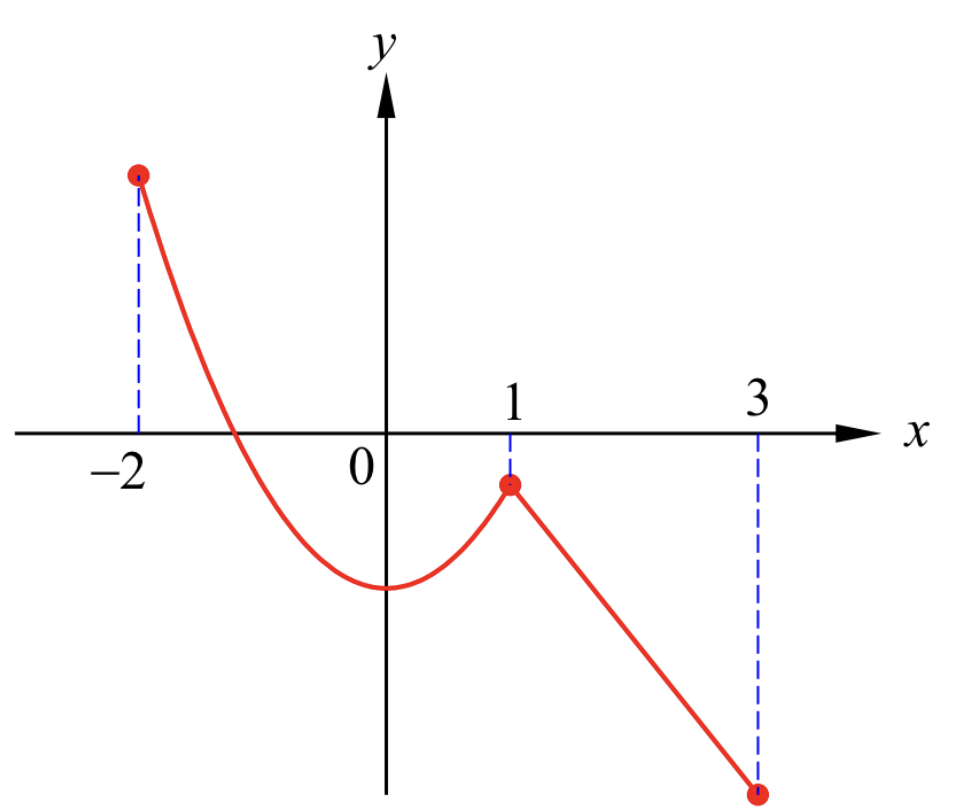
\includegraphics[scale=0.2]{Picture10.png}
\caption{  The function defined in Example \ref{23020902}.}\label{figure10}
\end{figure}

\begin{remark}{}
We can formulate a general theorem from Example \ref{23020902} as follows. 

Let $D$ be a subset of real numbers that contains the point $x_0$, and let $D_{x_0,-}$ and $D_{x_0,+}$ be the intersection of $D$ with the sets $\{x\,|\,x<x_0\}$ and $\{x\,|\,x>x_0\}$ respectively. Suppose that $x_0$ is a limit point of both $D_{x_0,-}$ and $D_{x_0, +}$, and $f:D\rightarrow\mathbb{R}$ is a function such that  its restrictions to $D_{x_0,-}$ and $D_{x_0, +}$ are continuous. If
\[\lim_{x\rightarrow x_0^-}f(x)=\lim_{x\rightarrow  x_0^+}f(x)=f(x_0),\] then $f:D\rightarrow\mathbb{R}$ is a continuous function.
\end{remark}

Finally, we define a special class of continuous functions called the Lipschitz function.

\begin{definition}{Lipschitz Function}
Let $D$ be a subset of real numbers. A function $f:D\rightarrow \mathbb{R}$ is said to be a Lipschitz function if there is a  constant $c$ such that
\[|f(x_1)-f(x_2)|\leq c|x_1-x_2|\hspace{1cm}\text{for all}\;x_1, x_2\in D.\]
The constant $c$ is called a Lipschitz constant of the function.
\end{definition}

Notice that a Lipschitz constant is nonnegative. The only  Lipschitz functions with 0 Lipschitz constant  are the constant functions. If $c_0$ is a Lipschitz constant of a Lipschitz function $f:D\rightarrow \mathbb{R}$, any number $c$ that is larger than $c_0$ is also a Lipschitz constant of $f$.

\begin{example}{}
Let $f:\mathbb{R}\rightarrow\mathbb{R}$ be the function given by $f(x)=ax+b$. Then $f$ is a Lipschitz function with Lipschitz constant $|a|$.
\end{example}

\begin{example}[label=23021007]{}
Let $f:[-10, 8]\rightarrow \mathbb{R}$ be the function defined by $f(x)=x^2$. Show that $f$ is Lipschitz.
\end{example}
\begin{solution}{Solution}
For any $x_1$ and $x_2$ in $[-10, 8]$, 
\[|f(x_1)-f(x_2)|=|x_1^2-x_2^2|=|x_1+x_2||x_1-x_2|.\]
Triangle inequality implies that
\[|x_1+x_2|\leq |x_1|+|x_2|\leq 10+10=20.\]
Hence,
\[|f(x_1)-f(x_2)|\leq 20|x_1-x_2|.\]
This shows that $f$ is a Lipschitz function with Lipschitz constant $20$.
\end{solution}

\begin{example}{}
Let $f:\mathbb{R}\rightarrow \mathbb{R}$ be the function defined by $f(x)=x^2$. Is $f$ a Lipschitz function?
\end{example}
\begin{solution}{Solution}
If $f$ is a Lipschitz function, there is a positive constant $c$ such that
\[|f(x_1)-f(x_2)|\leq c|x_1-x_2|\] for all real numbers $x_1$ and $x_2$. 
 Take   $x_1=c+1$ and $x_2=0$. We find that
\[(c+1)^2=|f(x_1)-f(x_2)|\leq c|x_1-x_2|= c(c+1),\] which implies that $c+1\leq 0$, a contradiction.
Hence, $f$ is not a Lipschitz function.
\end{solution}

Here we see that whether a function is Lipschitz or not depends on the domain.
Finally we prove that a Lipschitz function is continuous. 

\begin{theorem}[label=23021005]{}
Let $D$ be a subset of real numbers. If $f:D\rightarrow\mathbb{R}$ is a Lipschitz function, then it is continuous.
\end{theorem}
\begin{myproof}{Proof}
Since $f:D\rightarrow\mathbb{R}$ is Lipschitz,  there is a positive constant $c$ such that for any $x_1$ and $x_2$ in $D$,
\[|f(x_1)-f(x_2)|\leq c|x_1-x_2|.\]Let $x_0$ be a point in $D$. Given $\varepsilon>0$, take $\delta =\varepsilon/c$. Then $\delta>0$ and for any $x\in D$, if $|x-x_0|<\delta$,
\[|f(x)-f(x_0)|\leq c|x-x_0|<c\delta=\varepsilon.\] This proves that $f$ is continuous at $x_0$. Hence, $f:D\rightarrow\mathbb{R}$ is a continuous function.
\end{myproof}
\vp

\noindent
{\bf \large Exercises  \thesection}
\setcounter{myquestion}{1}



 \begin{question}{\themyquestion}
 Consider the function $f:\mathbb{R}\rightarrow\mathbb{R}$ defined by
 \[f(x)=\begin{cases} 2,\quad &\text{if}\;x>2,\\
 x,\quad & \text{if}\;x\leq 2\end{cases}.\]
 Show that $f$ is a continuous function.
\end{question}
\atc
 \begin{question}{\themyquestion}
  Consider the function $f:\mathbb{R}\rightarrow\mathbb{R}$ defined by
 \[f(x)=\begin{cases} x^2,\quad &\text{if $x$ is rational},\\
 -x^2,\quad & \text{if $x$ is irrational}.\end{cases}\]Show that $f$ is continuous at $x=0$.
 
\end{question}
\atc
 \begin{question}{\themyquestion}
  Consider the function $f:\mathbb{R}\rightarrow\mathbb{R}$ defined by
 \[f(x)=\begin{cases} 2x+5,\quad &\text{if}\;x<-1,\\
 ax^2+x,\quad & \text{if}\;x\geq -1\end{cases}.\]
 Show that there is a value of $a$ for which $f$ is a continuous function.
\end{question}
\atc
 \begin{question}{\themyquestion}
 Let $f:[-7, 5]\rightarrow\mathbb{R}$ be the function defined by $f(x)=2x^2+3x$. Show that $f$ is  a Lipschitz function.
\end{question}
\atc
 
 \begin{question}{\themyquestion}
Let $f:[1, \infty)\rightarrow \mathbb{R}$ be the function defined by $f(x)=\sqrt{x}$. Show that $f$ is a Lipschitz function.
\end{question}
\vp

\section{The Extreme Value Theorem}\label{sec2.3}
For a real-valued function $f:D\rightarrow\mathbb{R}$, the maximum value   is the largest  value the function can assume; while the minimum value  is the smallest value the function can assume.
\begin{definition}{Maximium and Minimum Values of a Function}
Let $D$  be a subset of real numbers. Given that $f:D\rightarrow\mathbb{R}$ is a  real-valued function  defined on $D$.
\begin{enumerate}[1.]
\item  $f$  has a maximum value if and only if there is a point $x_0$ in $D$ such that
\[f(x)\leq f(x_0)\hspace{1cm}\text{for all}\;x\in D.\]
Such a  $x_0$ is called a {\bf maximizer} of the function $f$.
\item  $f$  has a minimum value if and only if there is a point $x_0$ in $D$ such that
\[f(x)\geq f(x_0)\hspace{1cm}\text{for all}\;x\in D.\]
Such a  $x_0$ is called a {\bf minimizer} of the function $f$.
\end{enumerate}
\end{definition}

\begin{highlight}{Extreme Values}The maximum value of a function $f:D\rightarrow \mathbb{R}$ is the maximum of the set $f(D)$; while the minimum value is the minimum of the set $f(D)$.

A maximum value or a minimum value of a function  is called an {\bf extreme value} of the function. 
\end{highlight}

\begin{example}
[label=23020905]{}
\begin{enumerate}[(a)]
\item For the function $f:[-1, 2]\rightarrow \mathbb{R}$, $f(x)=2x$, $D=[-1,2]$ and $f(D)=[-2, 4]$. Thus, $f$ has minimum value $-2$ and maximum value 4.
\item For the function $g:[-1, 2)\rightarrow \mathbb{R}$, $g(x)=2x$, $D=[-1, 2)$ and $g(D)=[-2, 4)$. Thus, $g$ has minimum value $-2$, but it does not have maximum value.\end{enumerate}\be\begin{enumerate}[(a)]
\item[(c)] For the function $h:(-1, 2]\rightarrow \mathbb{R}$, $h(x)=2x$, $D=(-1, 2]$ and $h(D)=(-2, 4]$. Thus, $h$ has  maximum value 4, but it does not have minimum value.
\end{enumerate}
\end{example2}



 \begin{figure}[ht]
\centering
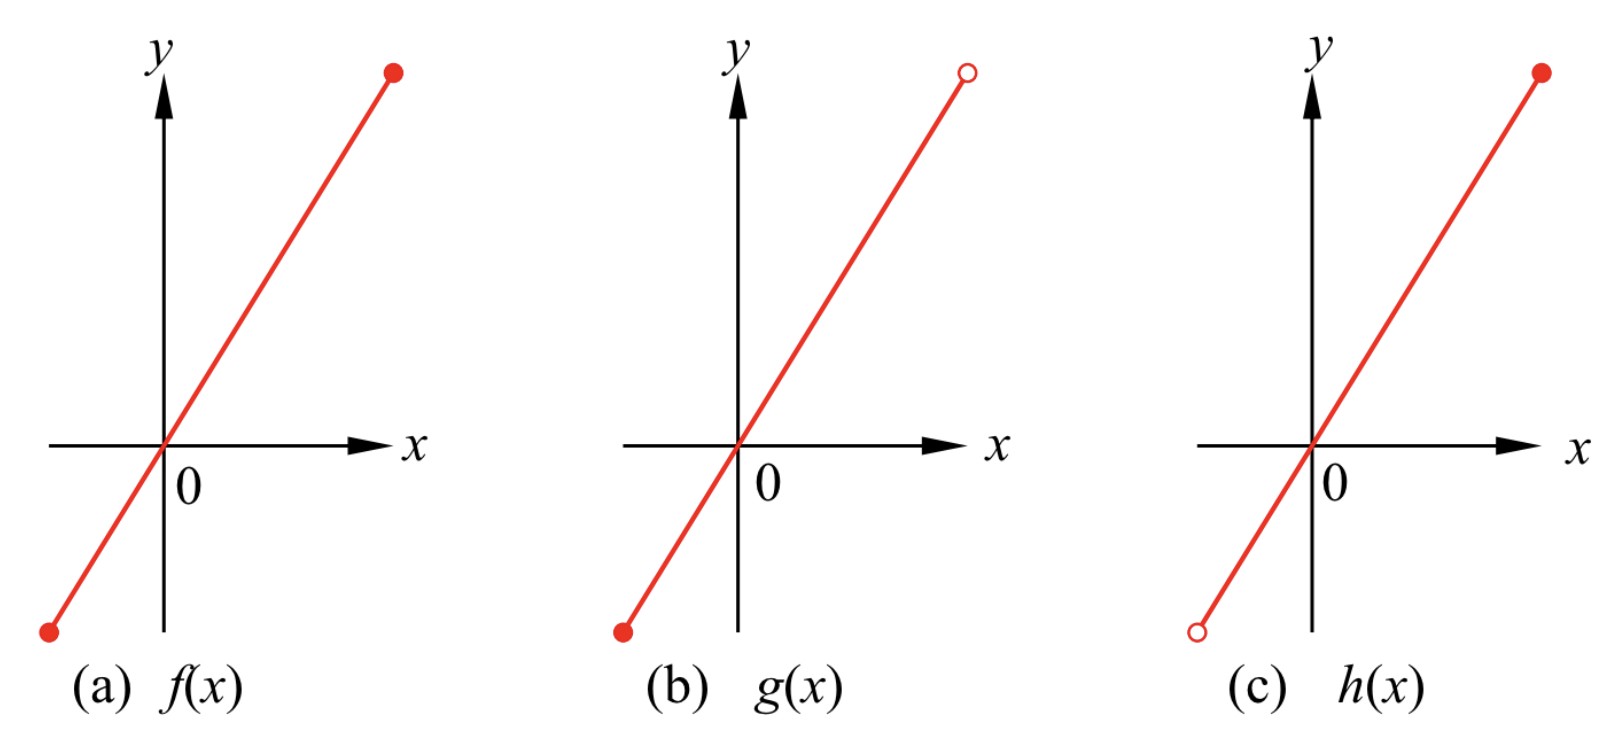
\includegraphics[scale=0.2]{Picture11.png}
\caption{  The functions $f(x)$, $g(x)$ and $h(x)$ defined in Example \ref{23020905}.}\label{figure11}
\end{figure}



Example \ref{23020905} shows that the existence of extreme values  depends on the domain of the function.

 


For a set to have maximum and minimum values, it is necessary (but not sufficient) that the set is bounded. Let us first define what it means for a function to be bounded.

\begin{definition}{Bounded Functions}
We say that a real-valued function $f:D\rightarrow\mathbb{R}$ is bounded if its range $f(D)$ is bounded. In other words, a function $f:D\rightarrow\mathbb{R}$ is bounded  if and only if there is a positive constant $M$ such that 
\[|f(x)|\leq M\hspace{1cm}\text{for all}\;x\in D.\]

\end{definition}

\begin{example}{}
All the three functions defined in Example \ref{23020905} are  bounded.
\end{example}



We are interested in a sufficient condition for a continuous function to have maximum and minimum values. Before we proceed, let us look at two examples.
 
 
  \begin{example}{}
 Consider the function $f:(0,1)\rightarrow\mathbb{R}$ defined by $\di f(x)=\frac{1}{x}$. Although the domain of the function $D=(0,1)$ is bounded, the range of the function $f(D)=(1, \infty)$ is not bounded.
 \end{example}
 This example shows that a continuous function does not necessarily map a bounded set to a bounded set. 
 
 
  \begin{example}{}
 Consider the function $f:[1,\infty)\rightarrow\mathbb{R}$ defined by $\di f(x)=\frac{1}{x}$. Although the domain of the function $D=[1, \infty)$ is closed, the range of the function $f(D)=(0, 1]$ is not closed.
 \end{example}
 This example shows that a continuous function does not necessarily map a closed set to a closed set. 
  
   The situation changes   when we combine closed and bounded.
 Recall that we have defined the concept of sequential compactness in Chapter \ref{ch1}, Section \ref{sec1.8}. A set $D$ is sequentially compact if    every sequence in $D$ has a subsequence that converges to a point in $D$. We have proved that a subset of real numbers is sequentially compact if and only if it is closed and bounded.
 

  The following theorem says that a continuous function maps a  closed and bounded set to a closed and bounded set.
 
  \begin{theorem}[label=23020906]{}
  Let $D$ be a closed and bounded subset of $\mathbb{R}$. If $f:D\rightarrow \mathbb{R}$ is  a continuous function, then the set $f(D)$ is   closed and bounded.
  \end{theorem}
  Using the fact that a subset of real numbers is sequentially compact if and only if it is closed and bounded, Theorem \ref{23020906} is equivalent to the following.
  \begin{theorem}
  [label=23020607]{}
  Let $D$ be a sequentially compact subset of $\mathbb{R}$. If $f:D\rightarrow \mathbb{R}$ is  a continuous function, then the set $f(D)$ is sequentially compact.
  \end{theorem}
  \begin{myproof}{Proof}
  We use the definition of sequential compactness to prove this theorem.  Let $\{y_n\}$ be a sequence in $f(D)$. We need to prove that there is a subsequence of $\{y_n\}$ that converges to a point in $f(D)$. 
  
  For each positive integer $n$, since $y_n$ is in $f(D)$, there is an $x_n$ in $D$ such that $f(x_n)=y_n$. This gives a sequence $\{x_n\}$ in $D$. Since $D$ is sequentially compact, there is a subsequence $\{x_{n_k}\}$ of $\{x_n\}$ that converges to a point $x_0$ in $D$. Since $f$ is continuous at $x_0$, the sequence $\{f(x_{n_k})\}$ converges to $f(x_0)$. In other words, we have shown that the subsequence $\{y_{n_k}\}$ of $\{y_n\}$ converges to the point $f(x_0)$ in $f(D)$.
 

  \end{myproof}
  
Proving Theorem \ref{23020906}   without using  sequential compactness is tedious, and it essentially goes through some of the arguments used to prove that a subset of real numbers is sequentially compact if and only if it is closed and bounded. From here, we can see the usefulness of the concept of sequential compactness.
  
  In Theorem \ref{23020908}, we have seen that a set that is closed and bounded must have a maximum and a minimum. Hence, we obtain immediately the following   theorem.
  
  \begin{theorem}[label=23020909]{Extreme Value Theorem}
 
  Let $D$ be a closed and bounded subset of $\mathbb{R}$. If $f:D\rightarrow \mathbb{R}$ is  a continuous function, then $f$ has a maximum value and a minimum value. 
    \end{theorem}
    \begin{corollary}{}
  If $f:[a,b]\rightarrow\mathbb{R}$ is a continuous function defined on a closed and bounded interval, then $f$ is bounded, and it has a maximum value and a minimum value. \end{corollary}

  
  Extreme value theorem is used to guarantee the existence of a maximum value and a minimum value before we proceed to find these values, so that the attempt to look for extreme values is not futile. In some circumstances, knowing the existence of such extreme values is sufficient. 
  
  \begin{example}{}
  Show that the function $f:\mathbb{R}\rightarrow\mathbb{R}$ defined by 
  \[f(x)=|x-1|+|x-2|+|x-3|+|x-4|+|x-5|\] has a minimum value. 
  \end{example}
  \begin{solution}{Solution}
  In this example, the domain of the function is not closed and bounded. We cannot apply the extreme value theorem directly. However, we can proceed in the following way.
  First, we justify that the function  $f:\mathbb{R}\rightarrow\mathbb{R}$  is continuous. A function of the form $g(x)=x-a$ is continuous since it is a polynomial. Absolute value of a continuous function is continuous. Hence, a function of the form $h(x)=|x-a|$ is continuous. Being a sum of continuous functions, $f(x)$ is a continuous function.

 To prove the existence of a minimum value,  we notice that for $x\geq 5$,
  \[f(x)=x-1+x-2+x-3+x-4+x-5=5x-15\geq  10.\]
  For $x\leq 1$,  
  \[f(x)=1-x+2-x+3-x+4-x+5-x=15-5x\geq 10.\]
  Now restrict the domain to $[1,5]$, the function $f:[1,5]\rightarrow\mathbb{R}$ is continuous. Hence, it has a minimum value at some $x_0\in [1,5]$. It follows that
  \[f(x_0)\leq f(x)\hspace{1cm}\text{for all}\;x\in [1,5].\]
  In particular,
  \[f(x_0)\leq f(1)=10.\] 
  This proves that for all $x\in\mathbb{R}$, 
$f(x)\geq f(x_0)$.
  Hence, the function $f:\mathbb{R}\rightarrow\mathbb{R}$ has a minimum value.
  \end{solution}
  
\vp
\noindent
{\bf \large Exercises  \thesection}
\setcounter{myquestion}{1}
 \begin{question}{\themyquestion}
 Determine whether the function is bounded.
 \begin{enumerate}[(a)]
 \item $f:\mathbb{R}\rightarrow\mathbb{R}$, $\di f(x)=\frac{x}{\sqrt{x^2+4}}$.
 \item $f:(0,1)\rightarrow\mathbb{R}$, $f(x)=x+\di\frac{1}{x}$.
 \end{enumerate}
\end{question}
\atc
 \begin{question}{\themyquestion}
 If a function $f:D\rightarrow\mathbb{R}$ is continuous and bounded, does it necessarily have a maximum value and a minimum value? Justfiy your answer.
\end{question}
\atc
 \begin{question}{\themyquestion}
 Let $f:[-4,4]\rightarrow\mathbb{R}$ be the function defined by 
 \[f(x)=\frac{x^2+x+1}{\sqrt{4x^2+9}}.\]Show that it has a maximum value and a minimum value.
\end{question}
\vp

\section{The Intermediate Value Theorem}\label{sec2.4}


In this section, we are going to discuss  the intermediate value theorem, which is an  important theorem for continuous functions. It is essentially a theorem about existence of solutions for equations defined by continuous functions. 

\begin{theorem}{Intermediate Value Theorem}
Given that $f:[a,b]\rightarrow \mathbb{R}$ is a continuous function. For any real number $w$ that is between $f(a)$ and $f(b)$, there exists a point $c$ in $[a, b]$ such that
\[f(c)=w.\]

\end{theorem}


\begin{myproof}{Proof}
The proof is using bisection method, which provides a constructive way to find the point $c$. 

Without loss of generality, assume that $f(a)<w<f(b)$.

We construct two sequences $\{a_n\}$ and $\{b_n\}$ recursively. Define $a_1=a$, $b_1=b$, and let
\[m_1=\frac{a_1+b_1}{2}\] be the midpoint of $a_1$ and $b_1$. The interval $[a,b]=[a_1, b_1]$ is bisected into two  subintervals $[a_1, m_1]$ and $[m_1, b_1]$ by the point $m_1$. 

 We want to define the interval $[a_2, b_2]$ to be one of these, based on the value of $f(m_1)$. 
\begin{enumerate}[$\bullet$\;\;]\item
If $f(m_1)<w$, define $a_2=m_1$ and $b_2=b_1$.
 \item If $f(m_1)\geq w$, define $a_2=a_1$ and $b_2=m_1$.
 
 \end{enumerate}By  definition,
 \[a_1\leq a_2<b_2\leq b_1,\]
 \[f(a_2)<w\leq f(b_2),\] and  the length of the interval $[a_2, b_2]$ is half the length of the interval $[a_1, b_1]$. 
 \bp
 Suppose that we have defined $a_1, \ldots, a_n$, $b_1, \ldots, b_n$, such that
 \[a_1\leq   \ldots \leq a_{n-1}\leq a_n<b_n\leq b_{n-1}\leq \ldots \leq b_1,\]
 \[f(a_k)<w\leq f(b_k)\hspace{1cm}\;\text{for all}\;1\leq k\leq n,\]
 and
 \[b_k-a_k=\frac{b_{k-1}-a_{k-1}}{2} \hspace{1cm} \text{for all}\;2\leq k\leq n.\]
 Let
 \[m_n=\frac{a_n+b_n}{2}\]  be the midpoint of $a_n$ and $b_n$.
 \begin{enumerate}[$\bullet$\;\;]\item
If $f(m_n)<w$, define $a_{n+1}=m_n$ and $b_{n+1}=b_n$.
 \item If $f(m_n)\geq w$, define $a_{n+1}=a_n$ and $b_{n+1}=m_n$.
 
 \end{enumerate}  By   definition,
 \[a_n\leq a_{n+1}<b_{n+1}\leq b_n,\]
 \[f(a_{n+1})<w\leq f(b_{n+1}),\] and  
 \[b_{n+1}-a_{n+1}=\frac{b_n-a_n}{2}.\]
This constructs the sequences $\{a_n\}$ and $\{b_n\}$. Notice that $\{a_n\}$ is an increasing sequence that is bounded above by $b$, while $\{b_n\}$ is a decreasing sequence that is bounded below by $a$.
 
By monotone convergence theorem, the sequence $\{a_n\}$ converges to a number $c_1=\sup\{a_n\}$ and the sequence $\{b_n\}$ converges to a number $c_2=\inf\{b_n\}$. By induction, we find that
\[b_n-a_n=\frac{b-a}{2^{n-1}}.\]Taking $n\rightarrow \infty$ limits, we conclude that
\[c_2-c_1=0.\]\bp
It follows that the number   $c=c_1=c_2$   satisfies
\begin{equation}\label{eq230210_1}a_n\leq c\leq b_n\hspace{1cm}\text{for all}\;n\in\mathbb{Z}^+,\end{equation}and 
\begin{equation}\label{eq230210_2}\lim_{n\rightarrow\infty}a_n=c=\lim_{n\rightarrow\infty}b_n.\end{equation}
Eq. \eqref{eq230210_1} shows that $c$ is in $[a,b]$. The continuity of the function $f$ and \eqref{eq230210_2} implies that
\[f(c)=\lim_{n\rightarrow \infty}f(a_n)=\lim_{n\rightarrow\infty}f(b_n).\]
Since \[f(a_n)<w \quad\text{and}\quad f(b_n)\geq w\hspace{1cm}\text{for all}\; n\in\mathbb{Z}^+,\]
we find that
\[f(c)\leq w\hspace{1cm}\text{and}\hspace{1cm}f(c)\geq w.\]
This proves that $f(c)=w$, and hence completes the proof of the theorem.


\end{myproof}


 \begin{figure}[ht]
\centering
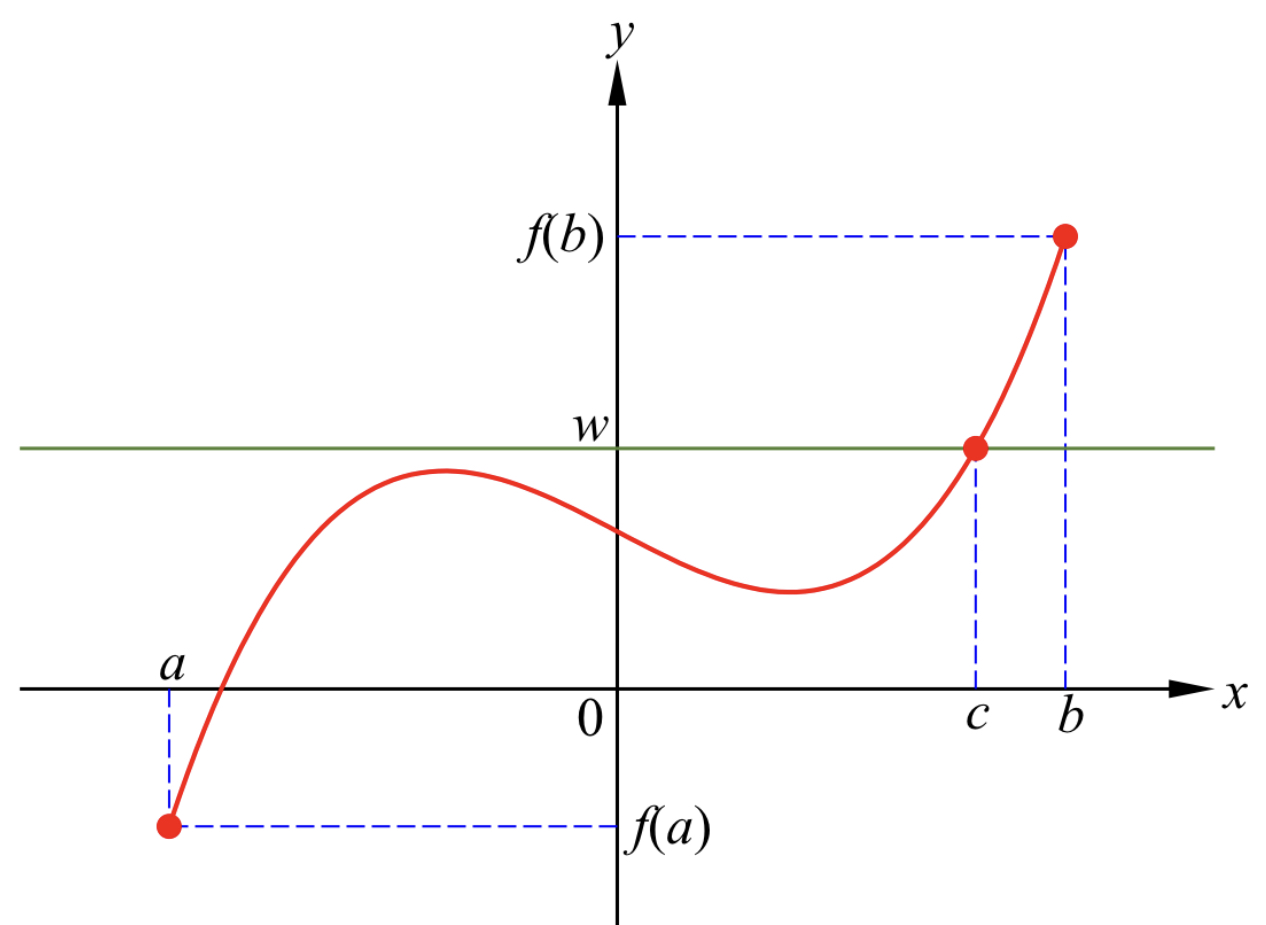
\includegraphics[scale=0.2]{Picture12.png}
\caption{The  intermediate value theorem.}\label{figure12}
\end{figure}
The following is an example which we use the intermediate value theorem to justify that an equation has a solution.
\begin{example}[label=ex230215_1]{}
Show that the equation 
\[x^6+6x+1=0\]has a real root.
\end{example}
\begin{solution}{Solution}
Let $f(x)=x^6+6x+1$.
Since $f(x)$ is a polynomial, it is a continuous function. Notice that
\[f(0)=1,\hspace{1cm}f(-1)=-4.\]
Hence, $f(-1)<0<f(0)$. Namely, $0$ is a value between $f(-1)$ and $f(0)$. By intermediate value theorem, there is a point $c$ in the interval $(-1,0)$ such that $f(c)=0$. Then $x=c$ is a root of the equation\[x^6+6x+1=0.\]
\end{solution}In this solution, the choice of $a=-1$ and $b=0$ are by trial and error. In practice, one can use a computer to sample some $x$ values and calculate the corresponding values of $f(x)$. The goal is to find   $a$ and   $b$ such that $f(a)$ and $f(b)$ have oppositive signs. To calculate the root $c$, one can implement the bisection method numerically.

\begin{example}{}
Let $n$ be a positive integer, and let $c$ be a positive number. Use the intermediate value theorem to show that there is a positive real number $x$ such that
\[x^n=c.\]
\end{example}

\begin{solution}{Solution}Take $a=0$, $b=c+1$, and
consider the function $f:[a, b]\rightarrow\mathbb{R}$ defined by $f(x)=x^n$. Then, \[f(a)=f(0)=0, \]
\[  f(b)=f(c+1)=(1+c)^n\geq 1+nc>c.\]
Hence, \[f(a)<c<f(b).\]
Since $f$ is a continuous function, intermediate value theorem asserts that there is a number $x$ in the interval $[0, c+1]$ such that $f(x)=x^n=c$.
\end{solution}
In Chapter \ref{ch1} Example \ref{23021011}, we use completeness axiom to solve this problem when $n=2$ and $c=2$. Here we use the intermediate value theorem to tackle the general problem. The tedious part has been settled in the proof of the intermediate value theorem.

In the following, we want to formulate a precise relation between intervals and the intermediate value theorem. We first introduce a concept called convexity.

\begin{definition}{Convex Sets}
Let $S$ be a subset of real numbers. We say that $S$ is convex if for any $u$ and $v$ in $S$, $(1-t)u+tv$ is in $S$ for all $t\in [0,1]$. \\Equivalently, $S$ is convex provided that whenever $u$ and $v$ are in $S$ and $u<v$, then any $w$ in the interval $[u,v]$ is also in $S$.
\end{definition}
The equivalence of the two definitions is seen by observing  that when $t$ changes from $0$ to $1$, $(1-t)u+tv$ goes through all the points in the interval $[u, v]$. 

Obviously, an interval is a convex set. The converse is also true.
\begin{theorem}{}
Let $S$ be a subset of real numbers. If $S$ is a convex set, then $S$ is an interval. 
\end{theorem}
\begin{myproof}{Sketch of Proof}
 If $S$ is bounded below, let $a=\inf S$. Otherwise, set $a=-\infty$. If $S$ is bounded above, let $b=\sup S$. Otherwise, set $b=\infty$. 

If $c$ is a point in $(a, b)$, then $a<c<b$. In particular, since $c>a$, it is not a lower bound of $S$. Hence, there is a point $u$ in $S$ such that $a\leq u<c$. Since $c<b$, $c$ is not an upper bound of $S$. Hence, there is a point $v$ in $S$ such that $c<v\leq b$. Since $u$ and $v$ are in $S$ and $S$ is convex, all points in the interval $[u,v]$ are in $S$. By construction, $u<c<v$. Hence, $c$ is in $S$. This proves that all the points in $(a, b)$ are in $S$.

 Finally, we just need to consider   whether $S$ contains $a$, and whether it contains $b$. 
\end{myproof}

\begin{highlight}{Convex Sets and Intervals}
Let $S$ be a convex set. If $S$ is bounded below, let $a=\inf S$.  If $S$ is bounded above, let $b=\sup S$.  
\begin{enumerate}[1.]
\item If $S$ is bounded, $S$ does not contain $\inf S$ and $\sup S$, then $S=(a,b)$.
\item If $S$ is bounded, $S$  contains $\inf S$ but does not contain $\sup S$, then $S=[a,b)$.
\item If $S$ is bounded, $S$  contains $\sup S$ but does not contain $\inf S$, then $S=(a,b]$.
\item If $S$ is bounded, and $S$  contains both $\inf S$ and $\sup S$, then $S=[a,b]$.
\item If $S$ is bounded below but not bounded above, and $S$ does not contain $\inf S$, then $S=(a,\infty)$.
\item If $S$ is bounded below but not bounded above, and $S$   contains $\inf S$, then $S=[a,\infty)$.
\end{enumerate}\begin{enumerate}[7.]
\item If $S$ is bounded above but not bounded below, and $S$ does not contain $\sup S$, then $S=(-\infty, b)$.
\end{enumerate}\end{highlight}\begin{highlight}{}\begin{enumerate}[8.]
\item If $S$ is bounded above but not bounded below, and $S$   contains $\sup S$, then $S=(-\infty, b]$.
\end{enumerate}\begin{enumerate}[9.]
\item If $S$ is not bounded above nor bounded below, then $S=(-\infty, \infty)=\mathbb{R}$.
\end{enumerate}
\end{highlight}

The following is a   reformulation of the intermediate value theorem.
\begin{theorem}{Intermediate Value Theorem}
Let $I$ be an interval. If the function $f:I\rightarrow\mathbb{R}$ is continuous, then $f(I)$ is an interval.
\end{theorem}
\begin{myproof}{Proof}
To show that $f(I)$ is an interval, take two distinct points $u$ and $v$ in $f(I)$. We need to show that any $w$ in between $u$ and $v$ is in $f(I)$. Since $u$ and $v$ are in $f(I)$, there exist $a$ and $b$ in $I$ such that $u=f(a)$ and $v=f(b)$. Without loss of generality, assume that $a<b$. Since $I$ is an interval, it contains the interval $[a,b]$. Since $f$ is continuous on $[a,b]$, and $w$ is in between $f(a)$ and $f(b)$,    the version of the intermediate value theorem that we have proved implies that there is a point $c$ in the interval $(a, b)$ such that $f(c)=w$. This shows that $w$ is also in $f(I)$.

 
\end{myproof}

\vp
\noindent
{\bf \large Exercises  \thesection}
\setcounter{myquestion}{1}
 \begin{question}{\themyquestion}
 Show that the equation 
$\di 2x+\sqrt{x^2+1}=0$ has a real solution.
\end{question}

\atc
\begin{question}{\themyquestion}
Given that $f:[-2, 10]\to [-2, 10]$ is a continuous function.
Show that there is a point $x$ in the interval $[-2, 10]$ such that $f(x)=x$.
\end{question}

\atc
\begin{question}{\themyquestion}
Suppose that $f:\mathbb{R}\rightarrow \mathbb{R}$ is a bounded continuous function.  Show that there is a real number $x$  such that $f(x)=x$.
\end{question}
\atc
\begin{question}{\themyquestion}
Let $n$ be an odd positive integer, and let \[p(x)=a_nx^n+a_{n-1}x^{n-1}+\cdots+a_1x+a_0\] be a polynomial of degree $n$. 
Show that $p(x)=0$ has a real root.
\end{question}
\vp

\section{Uniform Continuity}\label{sec2.5}
In Section \ref{sec2.2}, we have defined the concept of continuity at a point. This is a local property which only depends on the function value in a neighbourhood of a point. In this section, we want to define a concept called uniform continuity, which depends on the behaviour of the function on the whole domain. Such a property is called a global property.

\begin{definition}{Uniform Continuity}
Let $D$ be a subset of real numbers. A function  $f:D\rightarrow\mathbb{R}$  defined on $D$ is uniformly continuous provided that for any $\varepsilon>0$, there exists $\delta>0$ such that if $x_1$ and $x_2$ are in $D$ and $|x_1-x_2|<\delta$, then 
\[|f(x_1)-f(x_2)|<\varepsilon.\]
 
\end{definition}

\begin{theorem}[label=230404_1]{Equivalent Definition of Uniform Continuity}
Let $D$ be a subset of real numbers. A function  $f:D\rightarrow\mathbb{R}$  defined on $D$ is uniformly continuous if and only if whenever $\{u_n\}$ and $\{v_n\}$ are sequences in $D$ such that
\[\lim_{n\rightarrow\infty}(u_n-v_n)=0,\]
$\{f(u_n)\}$ and $\{f(v_n)\}$ are sequences in $f(D)$ such that
\[\lim_{n\rightarrow\infty}\Bigl(f(u_n)-f(v_n)\Bigr)=0.\] 
\end{theorem}
Notice that   we only require the sequence $\{u_n-v_n\}$ to converge to 0. We do not require the sequence $\{u_n\}$ nor the sequence $\{v_n\}$ to be convergent.

Theorem \ref{230404_1} can be proved in the same way as we prove the equivalence of two  definitions for limits of functions.

The following is quite obvious.
 \begin{theorem}[label=t23021006]{}
Let $D$ be a subset of real numbers. If $f:D\rightarrow\mathbb{R}$ is a  uniformly continuous function, it is continuous.
\end{theorem}



  Let us compare the definitions of continuity and uniform continuity using the definitions in terms of $\varepsilon-\delta$.

\begin{highlight}{Continuity versus Uniform Continuity}
\begin{enumerate}[$\bullet$]\item
A function $f:D\rightarrow \mathbb{R}$ is continuous if
\[\forall x_0\in D,\,\forall \varepsilon>0, \,\exists \delta>0,\, \forall x \in D, \, |x-x_0|<\delta\implies |f(x)-f(x_0)|<\varepsilon.\]
\item A function $f:D\rightarrow \mathbb{R}$  is uniformly continuous if
\[\forall \varepsilon>0, \,\exists \delta>0,\, \forall x_0\in D,\,\forall x \in D, \, |x-x_0|<\delta\implies |f(x)-f(x_0)|<\varepsilon.\]\end{enumerate}
\end{highlight}
The difference is in the order of the quantifiers. For a function to be continuous, it must be continuous at each point in the domain. For each point  $x_0$ in the domain, there should exist a positive $\delta$ for each positive $\varepsilon$. This number $\delta$ not only depends on $\varepsilon$, but also on the point $x_0$. For uniform continuity, one needs to be able to find a $\delta$ which only depends on $\varepsilon$ but not on the point in the domain. This is where the uniformity lies.

Let us look at some examples of functions that are continuous but not uniformly continuous.
\begin{example}{}
Show that the function $f:(0,1)\rightarrow\mathbb{R}$, $f(x)=\di\frac{1}{x}$ is not uniformly continuous. 
\end{example}
\begin{solution}{Solution}
For a positive integer $n$, let
\[u_n=\frac{1}{n+1},\hspace{1cm}v_n=\frac{1}{n+2}.\]
Then $\{u_n\}$ and $\{v_n\}$ are sequences in the domain $D=(0,1)$, and
\[\lim_{n\rightarrow\infty}(u_n-v_n)=\lim_{n\to\infty}\frac{1}{n+1}-\lim_{n\to\infty}\frac{1}{n+2}=0.\]\bs
Since $f(u_n)=n+1$ and $f(v_n)=n+2$, we find that
\[\lim_{n\rightarrow\infty}\Bigl(f(u_n)-f(v_n)\Bigr)=-1\neq 0.\]Hence, $f$ is not uniformly continuous.
\end{solution}

\begin{example}{}
Show that the function $f:(0,\infty)\rightarrow\mathbb{R}$, $f(x)=x^2$ is not uniformly continuous. 
\end{example}
\begin{solution}{Solution}
For a positive integer $n$, let
\[u_n=n+\frac{1}{n},\hspace{1cm}v_n=n.\]
Then $\{u_n\}$ and $\{v_n\}$ are sequences in the domain $D=(0,\infty)$, and
\[\lim_{n\rightarrow\infty}(u_n-v_n)=\lim_{n\rightarrow\infty}\frac{1}{n}=0.\] 
Since 
\[f(u_n)-f(v_n)=\left(n+\frac{1}{n}\right)^2-n^2=2+\frac{1}{n^2},\]we find that
\[\lim_{n\rightarrow\infty}\Bigl(f(u_n)-f(v_n)\Bigr)=2\neq 0.\]Hence, $f$ is not uniformly continuous.
\end{solution}

If we change the domain of the function, the conclusion is different.
\begin{example}[label=e23021008]{}
Let $f:[-10, 8]\rightarrow \mathbb{R}$ be the function defined by $f(x)=x^2$. Show that $f$ is uniformly continuous.
\end{example}
\begin{solution}{Solution}In the solution of Example \ref{23021007}, we have shown that
for any $x_1$ and $x_2$ in the domain $D=[-10, 8]$, 
\[|f(x_1)-f(x_2)|\leq 20|x_1-x_2|.\]
Given $\varepsilon>0$, take $\delta=\varepsilon/20$. Then $\delta>0$. If $x_1$ and $x_2$ are in $D$ and $|x_1-x_2|<\delta$, then
\[|f(x_1)-f(x_2)|<20\delta=\varepsilon.\]This proves that $f$ is uniformly continuous.
\end{solution}


Example \ref{e23021008} is a function that is Lipschitz. In fact, 
the proof of Theorem \ref{23021005} can be easily modified to prove that a Lipschitz function is uniformly continuous.
 \begin{theorem}[label=23021006]{}
Let $D$ be a subset of real numbers. If $f:D\rightarrow\mathbb{R}$ is a Lipschitz function, then it is uniformly continuous.
\end{theorem}

The converse is not true. For example, the function $f:[0,1]\rightarrow\mathbb{R}$, $f(x)=\sqrt{x}$ is not Lipschitz, but it is uniformly continuous. We leave this to the exercise. 


In the following, we give a sufficient condition for a function to be uniformly continuous. 
\begin{theorem}[label=23021008]{}
Let $D$ be a closed and bounded subset of real numbers. If $f:D\rightarrow\mathbb{R}$ is a continuous function, then it is uniformly continuous.
\end{theorem}
To prove this theorem, we start with a technical lemma.
\begin{lemma}[label=23021009]{}
Let $S$ be a sequentially compact set in $\mathbb{R}$, and let $\{a_n\}$ and $\{b_n\}$ be two sequences in $S$. There is strictly increasing sequence of positive integers $\{n_1, n_2, n_3,  \ldots\}$ such that each of 
 the subsequences  $\{a_{n_1}, a_{n_2}, a_{n_3}, \ldots\}$     and 
  $\{b_{n_1}, b_{n_2}, b_{n_3}, \ldots\}$    converges to a point in $S$.
\end{lemma}
Using sequential compactness, we can guarantee that $\{a_n\}$ has a subsequence  that converges to a point in $S$, and $\{b_n\}$ also has a subsequence that converges to a point in $S$. However, the indices of these two subsequences might not be related. We need to choose the subsequences carefully to make sure that the indices $\{n_k\}$ are the same. 
\begin{myproof}{Proof}
First, the sequentially compactness of $S$ guarantees that there is a strictly increasing sequence of positive integers  $\{k_1, k_2, k_3, \ldots\}$  so that the subsequence $\{a_{k_1}, a_{k_2}, a_{k_3}, \ldots\}$  converges to a point $a$ in $S$. For a positive integer $j$, let   
\[c_j=b_{k_j}.\] Consider the sequence $\{c_j\}$ indexed by $j\in\mathbb{Z}^+$. It is a subsequence of $\{b_n\}$, and it is also a sequence in $S$.  Since $S$ is sequentially compact, there is a strictly increasing sequence of positive  integers $\{j_1, j_2, j_3, \ldots\}$  such that the subsequence $\{c_{j_1}, c_{j_2}, c_{j_3}, \ldots\}=\{b_{k_{j_1}}, b_{k_{j_2}}, b_{k_{j_3}}, \ldots\}$ converges to a point $b$ in $S$. For a positive integer $m$, let
$\di n_m=k_{j_m}.$  Then $\{n_1, n_2, n_3, \ldots\}$ is a strictly increasing sequence of positive integers. The sequence $\{a_{n_1}, a_{n_2}, a_{n_3}, \ldots\}$ is a subsequence of $\{a_{k_1}, a_{k_2}, a_{k_3}, \ldots\}$. Hence, it converges to $a$. The sequence $\{b_{n_1}, b_{n_2}, b_{n_3}, \ldots\}$ is the sequence  $\{c_{j_1}, c_{j_2}, c_{j_3}, \ldots\}$ which converges to $b$.
\end{myproof}
Now we return to the proof of Theorem \ref{23021008}.
\begin{myproof}{\linkt Proof of Theorem \ref{23021008}}
We use proof by contradiction. If $f$ is not uniformly continuous,
there is an $\varepsilon>0$ such that for all $\delta>0$, there are points $u$ and $v$ is $D$ with $|u-v|<\delta$ and $|f(u)-f(v)|\geq\varepsilon$.
This implies that for each $n\in\mathbb{Z}^+$, there are points $u_n$ and $v_n$ in $D$ with 
\[\left|u_n-v_n\right|<\frac{1}{n}\quad \text{and}\quad\left|f(u_n)-f(v_n)\right|\geq\varepsilon.\]
Thus, $\{u_n\}$ and $\{v_n\}$ are two sequences in $D$ such that 
\begin{equation}\label{eq230210_5}\lim_{n\rightarrow\infty}(u_n-v_n)=0.\end{equation}
Since $D$ is closed and bounded, it is sequentially compact. By Lemma \ref{23021009}, we find that there is a strictly increasing sequence of positive integers $\{n_1, n_2, n_3,\ldots\}$ so that the subsequence $\{u_{n_k}\}$ converges to a point $u_0$ in $D$; and the subsequence $\{v_{n_k}\}$ converges to a point $v_0$ in $D$.  
 Since $f:D\to\mathbb{R}$ is continuous, the sequence $\{f(u_{n_k})\}$ converges to $f(u_0)$, and the sequence $\{f(v_{n_k})\}$  converges to $f(v_0)$.
By construction,
 \[|f(u_{n_k})-f(v_{n_k})|\geq \varepsilon\hspace{1cm}\text{for all}\;k\in\mathbb{Z}^+.\]
 This implies that
 \[|f(u_0)-f(v_0)|\geq \varepsilon.\]Since $\{u_{n_k}-v_{n_k}\}$ is a subsequence of $\{u_n-v_n\}$, \eqref{eq230210_5} implies that
\[u_0-v_0=\lim_{k\to\infty}\left(u_{n_k}-v_{n_k}\right)=0.\]
 In other words, $u_0=v_0$. Then we should have $f(u_0)=f(v_0)$, which contradicts to $|f(u_0)-f(v_0)|\geq\varepsilon$. 
We conclude that $f$ must be uniformly continuous.
\end{myproof}

\begin{example}{}
Show that the function $f:(0, 100)\rightarrow\mathbb{R}$, $f(x)=\sqrt{x}$ is uniformly continuous.
\end{example}
Using the definition of uniform continuity to solve this problem is tedious.
\begin{solution}{Solution}
The domain of the function $D_f=(0,100)$ is not closed and bounded. We cannot apply Theorem \ref{23021008} directly. Consider the function $g:[0,100]\rightarrow \mathbb{R}$ defined by $g(x)=\sqrt{x}$. It is a continuous function.
Since the domain $D_g=[0, 100]$ is closed and bounded, $g$ is uniformly continuous.

Since $f:(0, 100)\rightarrow\mathbb{R}$ is the restriction of the function $g$ to $D_f$, it is also uniformly continuous.
\end{solution}
\vspace{0.5cm}
\hrule
\vspace{0.5cm}
\noindent
{\bf \large Exercises  \thesection}
\setcounter{myquestion}{1}

\begin{question}{\themyquestion}
Determine whether the function $f:[0, \infty)\rightarrow \mathbb{R}$, $f(x)=2x^2+3x$ is uniformly continuous.
\end{question}
\atc
\begin{question}{\themyquestion}
Show that the function $f:(0, 20)\rightarrow \mathbb{R}$, $f(x)=\di\frac{x}{\sqrt{x+1}}$ is uniformly continuous.
\end{question}
\atc
 \begin{question}{\themyquestion}
Let $f:[0,1]\rightarrow\mathbb{R}$ be the function defined by $f(x)=\sqrt{x}$.
Show  that $f$ is not Lipschitz, but it is uniformly continuous.
\end{question}
\atc
\begin{question}{\themyquestion}
Determine whether the function $f:(0, 1)\rightarrow \mathbb{R}$, $f(x)=\di\frac{1}{\sqrt{x}}$ is uniformly continuous.
\end{question}



 
\vp


\section{Monotonic Functions and Inverses of  Functions}\label{sec2.6}

In this section, we study monotonic functions.
\begin{definition}{Monotonic    and Strictly Monotonic Functions}
Let $D$ be a subset of real functions and let $f:D\rightarrow\mathbb{R}$ be a function defined on $D$.
\begin{enumerate}[1.]
\item
We say that $f:D\to\mathbb{R}$ is an increasing function if for any $x_1$ and $x_2$ in $D$,
\[x_1\leq x_2\;\implies\;f(x_1)\leq f(x_2).\]
 
\item
We say that $f:D\to\mathbb{R}$ is a strictly increasing function if for any $x_1$ and $x_2$ in $D$,
\[x_1<x_2\;\implies\;f(x_1)< f(x_2).\]
 
\item
We say that $f:D\to\mathbb{R}$ is a decreasing function if for any $x_1$ and $x_2$ in $D$,
\[x_1\leq x_2\;\implies\;f(x_1)\geq f(x_2).\]
 \item
We say that $f:D\to\mathbb{R}$ is a strictly decreasing function if for any $x_1$ and $x_2$ in $D$,
\[x_1<x_2\;\implies\;f(x_1)> f(x_2).\]
\item We say that $f:D\to\mathbb{R}$ is monotonic if it is increasing or it is decreasing.
  

 
\item We say that $f:D\to\mathbb{R}$ is strictly monotonic if it is strictly increasing or it is strictly decreasing.
\end{enumerate}
\end{definition}
The following is obvious from the definitions.
\begin{proposition}{}
Let $D$ be a subset of real functions and let $f:D\rightarrow\mathbb{R}$ be a function defined on $D$. If $f$ is strictly monotonic, then it is one-to-one.
\end{proposition}
\begin{example}[label=23021101]{}\begin{enumerate}[(a)]
\item
Let $f:[-3,4]\rightarrow\mathbb{R}$  be the function defined by 
\[f(x)=\begin{cases} -1,\quad &\text{if}\;-3\leq x\leq 0,\\
x-1,\quad &\text{if}\hspace{0.5cm}0<x\leq 4.\end{cases}\]It is an increasing function.
\item Let   $g:[-3,4]\rightarrow\mathbb{R}$ be the function defined by 
\[g(x)=\begin{cases} 1,\quad &\text{if}\;-3\leq x\leq 0,\\
1-x,\quad &\text{if}\hspace{0.5cm}0< x\leq 4.\end{cases}\]It is a decreasing function. 
 \end{enumerate} Neither $f$ nor $g$ is strictly monotonic.
\end{example}

\begin{figure}[ht]
\centering
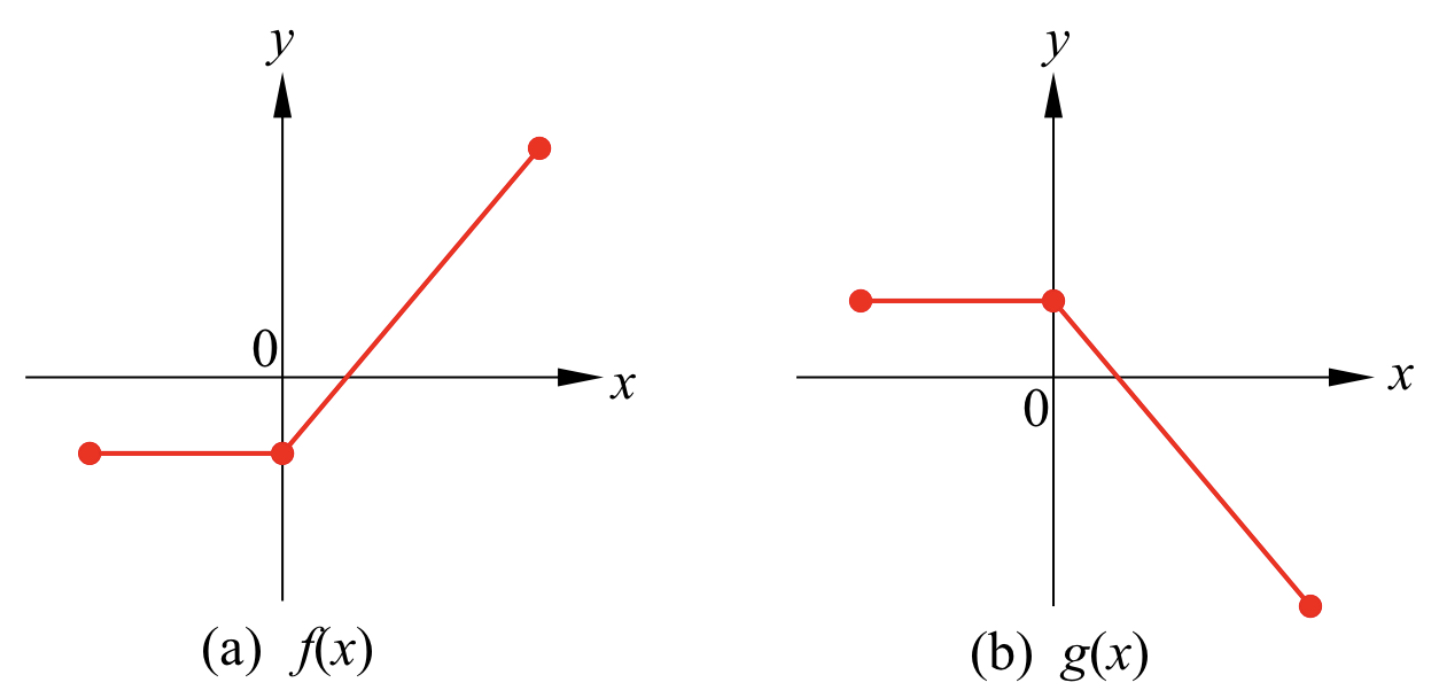
\includegraphics[scale=0.2]{Picture13.png}
\caption{  The functions $f(x)$ and $g(x)$ defined in Example \ref{23021101}.}\label{figure13}
\end{figure}

\begin{example}[label=23021102]{}
\begin{enumerate}[(a)]
\item Let $f:(-\infty, 0]\rightarrow\mathbb{R}$ be the function defined by $f(x)=x^2$. Then $f$ is strictly decreasing.

\item Let $g:[0, \infty)\rightarrow\mathbb{R}$ be the function defined by $g(x)=x^2$. Then $g$ is strictly increasing.\end{enumerate}
\end{example}


\begin{figure}[ht]
\centering
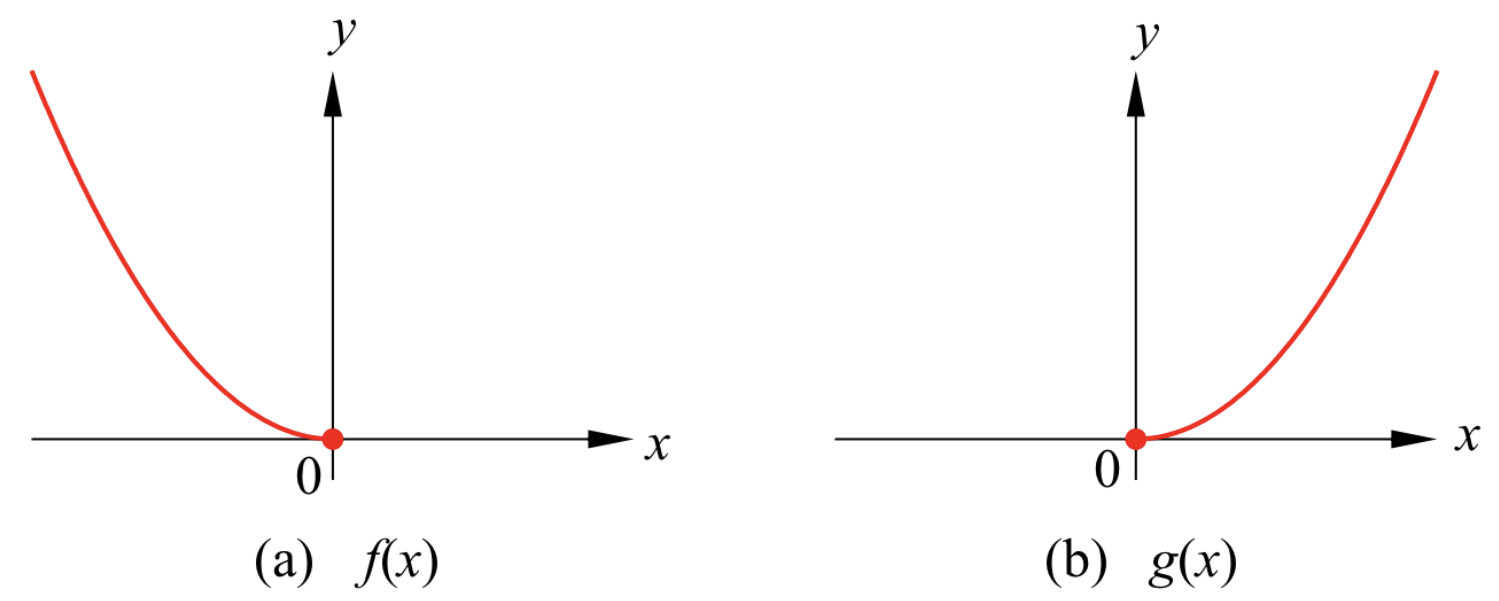
\includegraphics[scale=0.2]{Picture14.png}
\caption{  The functions $f(x)$ and $g(x)$ defined in Example \ref{23021102}.}\label{figure14}
\end{figure}





\begin{figure}[ht]
\centering
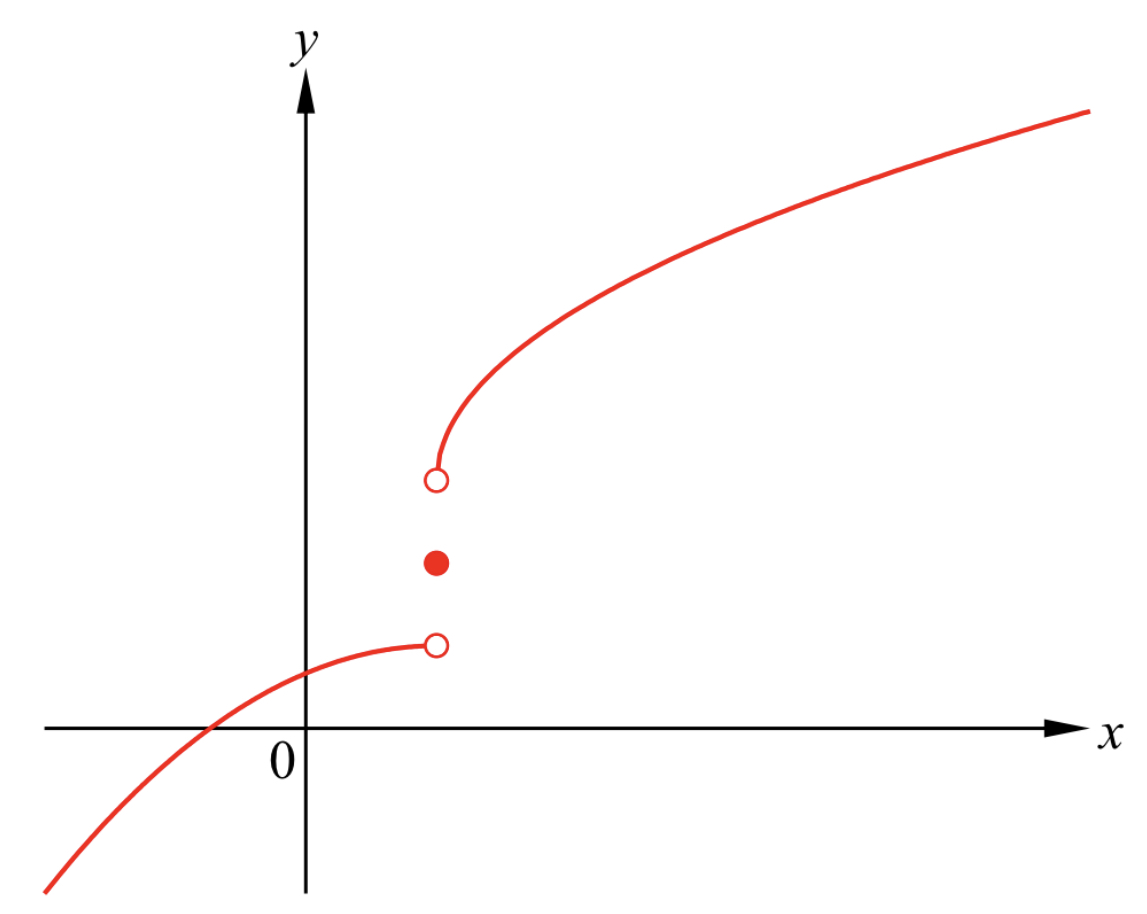
\includegraphics[scale=0.2]{Picture15.png}
\caption{  An increasing function with a jump discontinuity.}\label{figure15}
\end{figure}

\newpage

The following is a characterization of the discontinuities of a  monotonic function.
\begin{theorem}[label=23021103]{}
Let $f:[a,b]\rightarrow\mathbb{R}$ be a  monotonic function. For any $x_0$ in $(a, b]$, 
the left limit \[f_-(x_0)=\di \lim_{x\rightarrow x_0^-}f(x)\] exists. For any $x_0$ in $[a, b)$,    the right limit \[f_+(x_0)=\di\lim_{x\rightarrow x_0^+}f(x)\] exists. 
Define
\[f_-(a)=f(a)\quad\text{and}\quad f_+(b)=f(b).\] Then the  function $f:[a,b]\rightarrow\mathbb{R}$ is continuous at the point $x_0$ in $[a,b]$ if and only if 
\[f_-(x_0)=f(x_0)=f_+(x_0).\]
Otherwise, $f$ has a jump discontinuity at $x_0$ with jump \[|f_+(x_0)-f_-(x_0)|.\]
\end{theorem}


\begin{myproof}{Proof}
If $f$ is  decreasing, then $-f$ is  increasing. Hence, we only need to consider the case where  $f:[a,b]\rightarrow\mathbb{R}$  is  increasing.
Fixed $x_0$ in $(a, b]$. Define the nonempty set $S_-$ by
\[S_-=\left\{f(x)\,|\, a\leq x<x_0\right\}.\]
Since $f$ is  increasing,  $f(x)\leq f(x_0)$ for any $x$ in $[a, x_0)$. Therefore the set $S_-$ is bounded above by $f(x_0)$. Let $u=\sup S_-$. Then $u\leq f(x_0)$. 
We claim that
\[u=\di \lim_{x\rightarrow x_0^-}f(x)=f_-(x_0).\]
Given $\varepsilon>0$,  $u-\varepsilon <u$ and thus it is not an upper bound of $S_-$. Hence, there is a point $x_1$ in $[a, x_0)$ such that
\[f(x_1)>u- \varepsilon.\]\bp 
Let $\delta=x_0-x_1$. Then $\delta>0$. If $x$ is a point in $[a, x_0)$  such that $|x-x_0|<\delta$, then $x_1<x<x_0$, and thus
\[u-\varepsilon<f(x_1)\leq f(x)\leq u.\]From this, we have
\[|f(x)-u|<\varepsilon.\]This proves that
\[f_-(x_0)= \lim_{x\rightarrow x_0^-}f(x)=u.\]
Using similar argument, we find that for any $x_0$ in $[a, b)$, the right limit $\di\lim_{x\rightarrow x_0^+}f(x)$ exists, and
\[f_+(x_0)=\lim_{x\rightarrow x_0^+}f(x)=\inf \left\{f(x)\,|\, x_0<x\leq b\right\}.\]By definition of continuity, the function $f$ is continuous at $x_0$ if and only if $f_-(x_0)=f_+(x_0)$.
The statement about the jump is obvious.
 


\end{myproof}
 
\begin{corollary}[label=230222_1]{}
Let $I$ be an interval. If $f:I\rightarrow \mathbb{R}$ is monotonic, then $f$ is continuous if and only if $f(I)$ is an interval.
\end{corollary}


\begin{myproof}{Proof}
If $f:I\rightarrow \mathbb{R}$ is continuous, intermediate value theorem implies that $f(I)$ is an interval.

If $f:I\rightarrow \mathbb{R}$ is not continuous, Theorem \ref{23021103} implies that there is a point $x_0$ in the interval $I$ for which either $f_{-}(x_0)\neq f(x_0)$ or $f_+(x_0)\neq f(x_0)$. In any case, $f(I)$ cannot be an interval.
\end{myproof}

For a function $f:I\rightarrow\mathbb{R}$  defined on an interval $I$, we have seen that if $f$ is strictly monotonic, it is one-to-one. It is true even if the function is not continuous. If we assume that the function is continuous, the converse is also true.
It is a consequence of the intermediate value theorem.
\begin{theorem}[label=23021108]{}
Let $f:I\to \mathbb{R}$ be a function defined on an interval $I$. If $f$ is continuous and one-to-one, then $f$ is strictly monotonic. 
\end{theorem}
\begin{myproof}{Proof}
If $f$  fails to be strictly monotonic, there   exist three points $a, x_0, b$ in $I$ such that $a<x_0<b$ and one of the following holds.
\begin{enumerate}[(i)]
\item  $f(a)<f(b)<f(x_0)$
\item $f(x_0)<f(a)<f(b)$
\item $f(a)>f(b)>f(x_0)$
\item $f(x_0)>f(a)>f(b)$

\end{enumerate}Consider case (i) where $f(a)<f(b)<f(x_0)$. Since $w=f(b)$ is a value between $f(a)$ and $f(x_0)$, intermediate value theorem implies that there is a point $c$ in the interval $(a, x_0)$ for which $f(c)=w$. But then $c\neq b$, but $f(c)=f(b)$. This contradicts to $f$ is one-to-one.

Using the same argument, we will reach a contradiction for the other three cases. 
This proves that $f$ must be strictly monotonic.
\end{myproof}

Now we consider invertibility of functions. We only consider functions that are defined on intervals.
\begin{definition}{Invertibility of a Function}
Let  $I$ be an interval and let $f:I\rightarrow\mathbb{R}$ be a function defined on $I$. The function $f:I\rightarrow\mathbb{R}$ is invertible if and only if it is injective. If $f:I\rightarrow\mathbb{R}$ is injective,   its inverse is the function $f^{-1}:f(I)\rightarrow\mathbb{R}$ defined in such a way so that
\[f^{-1}(y)=x\iff f(x)=y\hspace{1cm}\text{for all}\;y\in f(I).\]
\end{definition}

\begin{example}[label=23021105]{}
Consider the functions $f$ and $g$ that are defined in Example \ref{23021102}. 
\begin{enumerate}[(a)]
\item The inverse of the function
  $f:(-\infty, 0]\rightarrow\mathbb{R}$, $f(x)=x^2$, is the function $f^{-1}:[0, \infty)\to (-\infty, 0]$, $f^{-1}(x)=-\sqrt{x}$.
\item The inverse of the function
$g:[0, \infty)\rightarrow\mathbb{R}$, $g(x)=x^2$, is the function $g^{-1}:[0, \infty)\to [0, \infty)$, $g^{-1}(x)=\sqrt{x}$.\end{enumerate}
\end{example}
\begin{figure}[ht]
\centering
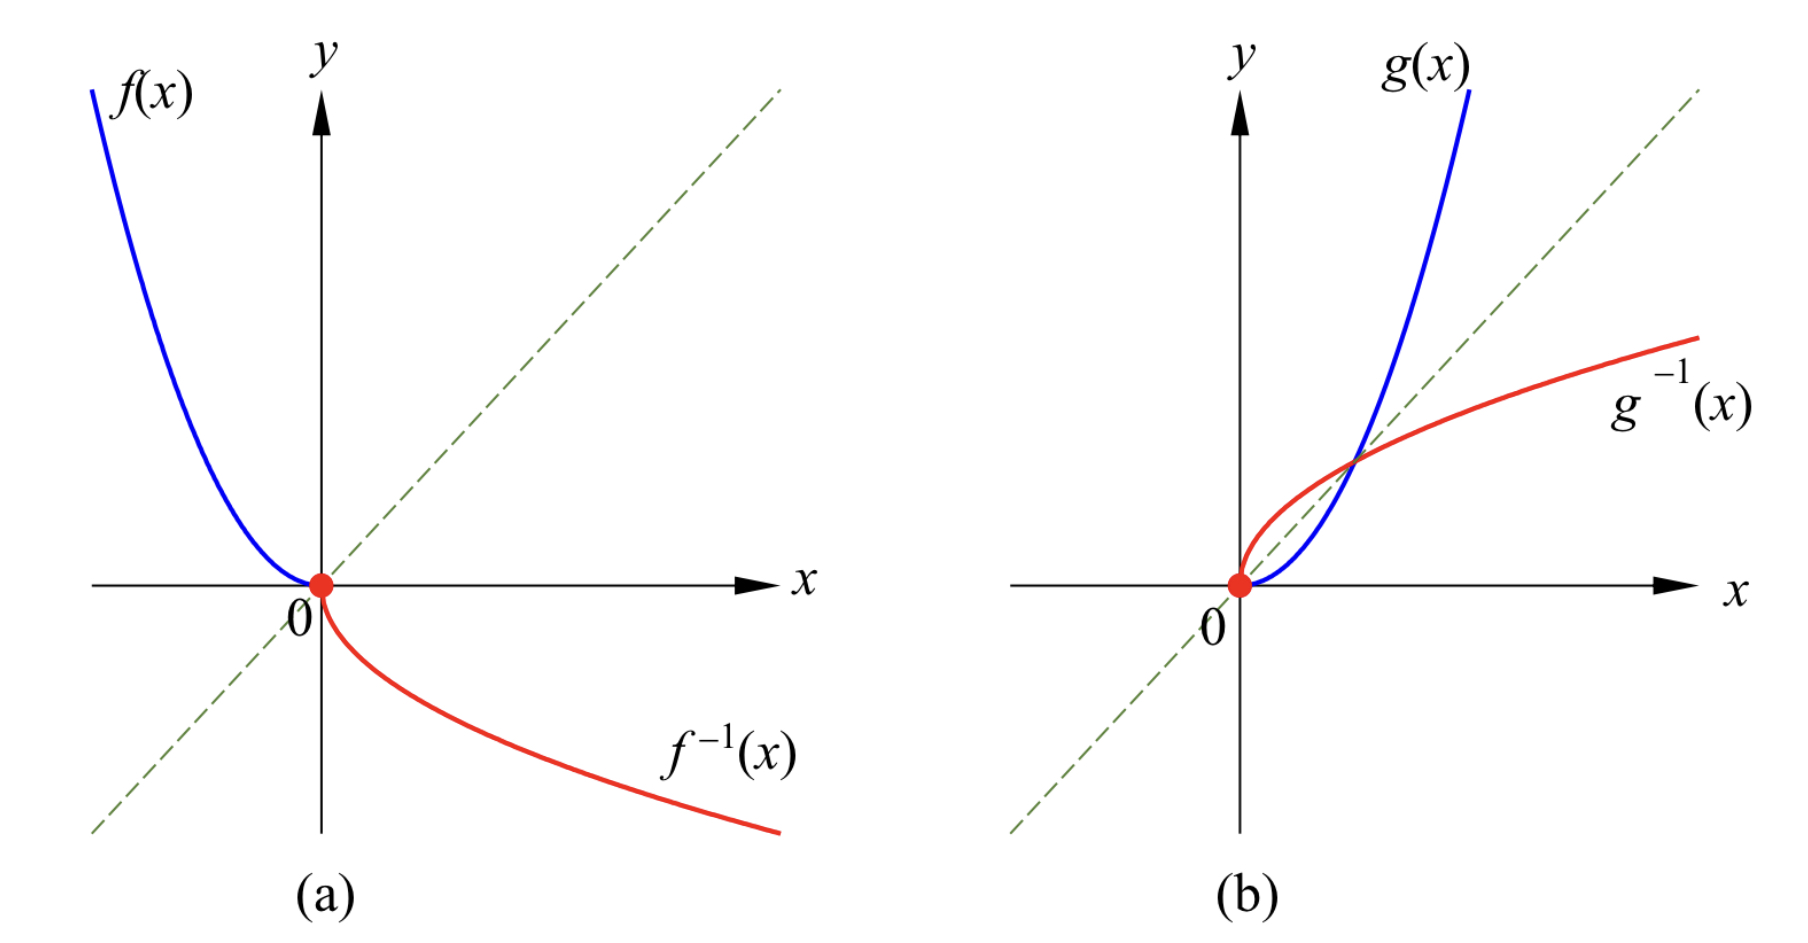
\includegraphics[scale=0.2]{Picture16.png}
\caption{  The functions  in Example \ref{23021105}.}\label{figure16}
\end{figure}
Notice that the inverse of a strictly increasing function is strictly increasing. The inverse of a strictly decreasing function is strictly decreasing.


In the next theorem, we prove that the inverse of a continuous function   is continuous. 
\begin{theorem}[label=23021106]{}
Let $I$ be an interval and let $f:I\to\mathbb{R}$ be a continuous function defined on $I$. If $f:I\rightarrow\mathbb{R}$ is one-to-one, then $f^{-1}:f(I)\to\mathbb{R}$ exists, and it is continuous.


\end{theorem}
\begin{myproof}
{Proof}
By Theorem \ref{23021108}, $f$ is strictly monotonic. Without loss of generality, we assume that $f$ is strictly increasing. 

 Given  a point $y_0$ in the interval $f(I)$, let $x_0$ be the unique point in $I$ such that $f(x_0)=y_0$. Given $\varepsilon>0$, we need to prove that there is a $\delta>0$ such that if $y$ is a point in $f(I)$ with $|y-y_0|<\delta$, then $|f^{-1}(y)-f^{-1}(y_0)|<\varepsilon$.

For simplicity, assume that $x_0$ is an interior point of $I$. Then there is a $r>0$ such that $[x_0-r,x_0+r]$ is in $I$. 
Take \[\varepsilon_1=\min\{\varepsilon, r\}.\] Then $\varepsilon_1>0$, $\varepsilon_1\leq \varepsilon$ and $[x_0-\varepsilon_1, x_0+\varepsilon_1]\subset [x_0-r, x_0+r]\subset I$.
Since $f$ is strictly increasing,
\[f(x_0-\varepsilon_1)<f(x_0)<f(x_0+\varepsilon_1),\]and the interval $[f(x_0-\varepsilon_1), f(x_0+\varepsilon_1)]$ is in $f(I)$. 
Let
\[\delta=\min\{f(x_0)-f(x_0-\varepsilon_1), f(x_0+\varepsilon_1)-f(x_0)\}.\]
Then $\delta>0$. If $y$ is a point in $I$ such that $|y-y_0|<\delta$, then \[f(x_0-\varepsilon_1)\leq y_0-\delta<y<y_0+\delta\leq f(x_0+\varepsilon_1).\]This implies that $y$ is also in $f(I)$.  Since $f^{-1}$ is  strictly increasing, we have
\[x_0-\varepsilon\leq x_0-\varepsilon_1<f^{-1}(y)<x_0+\varepsilon_1\leq x_0+\varepsilon.\]This implies that
\[|f^{-1}(y)-f^{-1}(y_0)|<\varepsilon,\]which completes the proof that $f^{-1}$ is continuous at $y_0$.

If $f^{-1}(y_0)=x_0$ is an endpoint of $I$, we need to modify the proof a bit to show that $f^{-1}$ is continuous at $y_0$. The details are left to the students.

\end{myproof}

\begin{remark}{}
If $I=(a, b)$ is an open interval and the function $f:(a, b)\to \mathbb{R}$ is continuous and one-to-one, we have seen in Theorem \ref{23021108} that $f$ is strictly monotonic. In fact, one can prove that $f(I)$ is also an open interval. 

Without loss of generality, assume that $f$ is strictly increasing.   Since $f$ is continuous, $f(I)$ is an interval. If $f(I)$ is not an open interval, either $\inf f(I)$ or $\sup f(I)$ is in $f(I)$. If $c=\inf f(I)$ is in $f(I)$, there is a point $u$ in $(a, b)$ such that $f(u)=c$. But then $u>a$ and so $u_1=\di \frac{u+a}{2}$ is also a point in $(a,b)$. Since $u_1<u$, $f(u_1)<f(u)=c$. This contradicts to $c=\inf f(I)$. In the same way, one can show that $\sup f(I)$ is not in $f(I)$. Hence, $f(I)$ must be an open interval.
\end{remark}

Although we can use limits to show that when $n$ is a positive integer, the  function $f(x)=\sqrt[n]{x}$ is continuous, it is tedious. Using Theorem \ref{23021106} is much more succint.
\begin{example}{}
Let $n$ be a positive integer. 
\begin{enumerate}[1.]
\item If $n$ is odd, the function $f:\mathbb{R}\to\mathbb{R}$, $f(x)=x^n$ is continuous and  one-to-one. Hence, its inverse
$f^{-1}:\mathbb{R}\to\mathbb{R}$, $f^{-1}(x)=\sqrt[n]{x}$ is a continuous function.
\item If $n$ is even, the function $f:[0,\infty)\to[0,\infty)$, $f(x)=x^n$ is continuous and  one-to-one. Hence, its inverse
$f^{-1}:[0,\infty)\to[0,\infty)$, $f^{-1}(x)=\sqrt[n]{x}$ is a continuous function.
\end{enumerate}
\end{example}


Recall that a rational number $r$ can be written as $r=p/q$, where $p$ is an integer and $q$ is a positive integer. For a positive real number $x$, we define
$x^r$ by
\[x^r=\sqrt[q]{x^p}=\left(\sqrt[q]{x}\right)^p.\]
It is easy to check that the two expressions for $x^r$ are equal.
Using the fact that composition of continuous functions is continuous, we obtain the following.

\begin{theorem}{}
Let $r$ be a rational number. 
\begin{enumerate}[1.]
\item If $r>0$, $f:[0,\infty)\to [0,\infty)$, $f(x)=x^r$ is a strictly increasing continuous function.
\item If $r<0$, $f:(0,\infty)\to (0,\infty)$, $f(x)=x^r$ is a strictly decreasing continuous function.
\end{enumerate}
\end{theorem}

\vspace{0.8cm}\hrule\vspace{0.8cm}
\noindent
{\bf \large Exercises  \thesection}
\setcounter{myquestion}{1}
 \begin{question}{\themyquestion}
 Show that the function $f:(-1,\infty)\rightarrow \mathbb{R}$, 
$\di f(x)=\frac{2x+1}{x+1}$ is strictly monotonic, and find  the inverse function $f^{-1}$.
\end{question}


